% Options for packages loaded elsewhere
\PassOptionsToPackage{unicode}{hyperref}
\PassOptionsToPackage{hyphens}{url}
%
\documentclass[
]{article}
\usepackage{amsmath,amssymb}
\usepackage{iftex}
\ifPDFTeX
  \usepackage[T1]{fontenc}
  \usepackage[utf8]{inputenc}
  \usepackage{textcomp} % provide euro and other symbols
\else % if luatex or xetex
  \usepackage{unicode-math} % this also loads fontspec
  \defaultfontfeatures{Scale=MatchLowercase}
  \defaultfontfeatures[\rmfamily]{Ligatures=TeX,Scale=1}
\fi
\usepackage{lmodern}
\ifPDFTeX\else
  % xetex/luatex font selection
\fi
% Use upquote if available, for straight quotes in verbatim environments
\IfFileExists{upquote.sty}{\usepackage{upquote}}{}
\IfFileExists{microtype.sty}{% use microtype if available
  \usepackage[]{microtype}
  \UseMicrotypeSet[protrusion]{basicmath} % disable protrusion for tt fonts
}{}
\makeatletter
\@ifundefined{KOMAClassName}{% if non-KOMA class
  \IfFileExists{parskip.sty}{%
    \usepackage{parskip}
  }{% else
    \setlength{\parindent}{0pt}
    \setlength{\parskip}{6pt plus 2pt minus 1pt}}
}{% if KOMA class
  \KOMAoptions{parskip=half}}
\makeatother
\usepackage{xcolor}
\usepackage[margin=1in]{geometry}
\usepackage{longtable,booktabs,array}
\usepackage{calc} % for calculating minipage widths
% Correct order of tables after \paragraph or \subparagraph
\usepackage{etoolbox}
\makeatletter
\patchcmd\longtable{\par}{\if@noskipsec\mbox{}\fi\par}{}{}
\makeatother
% Allow footnotes in longtable head/foot
\IfFileExists{footnotehyper.sty}{\usepackage{footnotehyper}}{\usepackage{footnote}}
\makesavenoteenv{longtable}
\usepackage{graphicx}
\makeatletter
\def\maxwidth{\ifdim\Gin@nat@width>\linewidth\linewidth\else\Gin@nat@width\fi}
\def\maxheight{\ifdim\Gin@nat@height>\textheight\textheight\else\Gin@nat@height\fi}
\makeatother
% Scale images if necessary, so that they will not overflow the page
% margins by default, and it is still possible to overwrite the defaults
% using explicit options in \includegraphics[width, height, ...]{}
\setkeys{Gin}{width=\maxwidth,height=\maxheight,keepaspectratio}
% Set default figure placement to htbp
\makeatletter
\def\fps@figure{htbp}
\makeatother
\setlength{\emergencystretch}{3em} % prevent overfull lines
\providecommand{\tightlist}{%
  \setlength{\itemsep}{0pt}\setlength{\parskip}{0pt}}
\setcounter{secnumdepth}{-\maxdimen} % remove section numbering
\ifLuaTeX
  \usepackage{selnolig}  % disable illegal ligatures
\fi
\IfFileExists{bookmark.sty}{\usepackage{bookmark}}{\usepackage{hyperref}}
\IfFileExists{xurl.sty}{\usepackage{xurl}}{} % add URL line breaks if available
\urlstyle{same}
\hypersetup{
  pdftitle={Funding Report: Goldberg Gator Engineering Explorers Summer Program 2023},
  pdfauthor={Krista D. Chisholm},
  hidelinks,
  pdfcreator={LaTeX via pandoc}}

\title{Funding Report: Goldberg Gator Engineering Explorers Summer
Program 2023}
\author{Krista D. Chisholm}
\date{October 19, 2023}

\begin{document}
\maketitle

{
\setcounter{tocdepth}{2}
\tableofcontents
}
\hypertarget{summary}{%
\section{Summary}\label{summary}}

The Goldberg Gator Engineering Explorers (GGEE) Summer Program was
designed to provide middle school students with an authentic experience
in programming, engineering design, and computational thinking. The 2023
Summer Program successfully engaged 319 students across 8 school
districts. Students developed computational thinking skills through
design-based challenges using micro:bit micro-controllers.

Schools and Districts partnered with the GGEE program to host programs
and sponsor teachers and materials for the programs at their schools.
There were 20 local teachers that lead summer programs in their area.
Twenty undergraduate engineering students from the University of Florida
and neighboring colleges and universities supported teacher leaders and
served as mentors for students in the program. Both teachers and
undergraduate mentors were trained in program activities to upskill
their abilities in programming, computational thinking, engineering
design, and teaching practices. Two grant staff coordinated and ran the
programs.

In addition to the funding from donors Arnold Goldberg and Bud and Kim
Deffebach, school districts, or city programs - City of Riviera Beach
Youth Empowerment Programs; the Goldberg Gator Engineering Explorers
summer programs received funding from the State of Florida Department of
Education (291-1231C-2C001) to aid in supporting student travel, time,
and providing technology.

\textbf{Last year summary} \emph{Students reported they felt challenged
during the program but were rewarded when their code or design worked.
They also mentioned the importance of collaboration with peers to solve
engineering problems, and they enjoyed the mentorship of the college
students working with the program. The longitudinal effects of the
summer program on grades in math and science and students' enrollment in
higher-level courses will be tracked by the research study for the
program. All districts provided in-kind donations to the camp, and many
school districts have plans to host or expand the programs for next
year. Some schools have asked about follow-up programming, including
afterschool programming to continue student engagement. The cost per
student for the program was \$996, including all costs for program
development (three months), camp costs (two months), and post-assessment
of the program. The cost per student for future camps should be less
owing to development costs built into the program's first year.}

\hypertarget{introduction}{%
\section{Introduction}\label{introduction}}

\hypertarget{background}{%
\subsection{Background}\label{background}}

The Goldberg Gator Engineering Explorers (GGEE) Summer Program was
initiated by a generous donor, Arnold Goldberg, to the University of
Florida Foundation. He envisioned a free summer program for
underrepresented minority middle school students. The program would
allow students and teachers to experience computer science and have
opportunities to learn to not only program but build skills in
computational thinking, problem solving, and engineering design. The
vision was brought to life by the Engaging Quality Instruction through
Professional Development (EQuIPD) grant at the University of Florida.
Their team worked with schools, districts, and teachers across Florida
to host these programs.

The GGEE Program was designed to introduce middle school-aged students
to programming and computer science. The program begins with students
learning the base elements of coding through small activities that
engage them in applying concepts such as strings, conditional
statements, loops, and variables. They use these concepts and the
micro:bit to develop a simple game and to also collect and analyze light
intensity data to study the relationship of light intensity and
distance. The program then has students working on two scaling design
challenges with partners and teams. The first is a creative engineering
design challenge where they create a micro:bit pet for a partner. Then
second is a technical design challenge where teams create a solution to
a local problem - traffic lights for emergency service vehicles,
environmental sensors for a farmer, and an indicator for new drivers.

An Advanced Program was developed and piloted during the second year of
the GGEE programs to allow returning students to continue to participate
in the GGEE programs. The program was designed to introduce students to
the basic concepts of Artificial Intelligence with a focus in Machine
Learning. The Advanced Program session designed to be held over 4
full-days where students began with basic ideas of artificial
intelligence and machine learning and are the scaffolded to developing
basic and more complex machine learning models that are trained from
text, images, and even gestures. This program was open to students who
previously attended the GGEE program in 2022.

\hypertarget{purpose-of-the-report}{%
\subsection{Purpose of the Report}\label{purpose-of-the-report}}

The purpose of this report is to offer a comprehensive overview of the
2023 Goldberg Gator Engineering Explorer Summer Programs. Through this
report, we aim to provide readers with insights into the entire
lifecycle of our summer programs, starting from the preparations leading
up to the program's launch, the activities and experiences that
transpired throughout the summer, and essential information pertaining
to post-program activities. Furthermore, this report will offer valuable
suggestions and recommendations for improving and enhancing the quality
and effectiveness of our future summer programs, setting the stage for
continued growth and success in the years to come.

\hypertarget{preparation}{%
\section{Preparation}\label{preparation}}

In preparation for the GGEE Summer Programs, the EQuIPD team actively
engaged in district recruitment, student enrollment, and the meticulous
preparation of essential research and compliance documentation.

\hypertarget{funding}{%
\subsection{Funding}\label{funding}}

Funding for the Goldberg Gator Engineering Explorer Summer Programs came
few multiple sources this year in addition to donation from Arnold
Goldberg to the University of Florida's Herbert Wertheim College of
Engineering.

\emph{State of Florida Department of Education}

The State of Florida Department of Education provided \$199,000
(291-1231C-2C001) to support the Goldberg Gator Engineering Explorer
Summer Programs alongside providing training and materials for teachers
around artificial intelligence. These funds supported staff time and
effort, program travel, technology, and consumable materials.

\emph{Bud and Kim Deffebach UF Foundation}

We partnered with Bud and Kim Deffebach to host both a GGEE summer
program and after-school program for students in Brevard County at Stone
Magnet Middle School. Their gift of \$24,000 provided funding for the
teacher to train and lead the summer and after-school programs,
consumable materials, technology, and meals for the students and staff
that participated in the summer program.

\emph{City of Riviera Beach - Youth Empowerment Programs}

The EQuIPD grant worked with the City of Riviera Beach to host a session
of the GGEE program over the summer. The city provided meals for the
students and a learning lab space for their Youth Empowerment Programs
within their public library. A \$5,500 contract was developed between UF
and the city for the city to provide funding for a teacher, technology,
and consumable learning materials. The GGEE program provided funding for
the student mentors supporting the program.

\emph{Schools and Districts}

Many of the schools and districts we collaborated with to host GGEE
summer programs were able to allocated funds from the end of the year to
support their teachers through training and leading sessions, technology
such as micro:bits and STEM kits for the teachers to keep for their own
classrooms and after-school programs, and consumable materials such as
paper, pencils, pens, markers, tape, and glue. The GGEE program provided
funding for student mentors time and any travel costs. Many school
districts provided breakfast and lunch for students participating in the
program as part of the already existing summer lunch programs. The
estimated costs for schools were around \$4,000 for 4-day programs and
around \$6,000 for 8-day half-day programs.

Table 1 displays the funding sources for each of the GGEE program
sessions. A more concise breakdown of funds will be provided in an
additional report.

\begin{longtable}[]{@{}llc@{}}
\caption{2023 Goldberg Gator Engineering Summer Program location funding
sources.}\tabularnewline
\toprule\noalign{}
School District & Program Funding Sources & Number of Programs \\
\midrule\noalign{}
\endfirsthead
\toprule\noalign{}
School District & Program Funding Sources & Number of Programs \\
\midrule\noalign{}
\endhead
\bottomrule\noalign{}
\endlastfoot
Alachua County Schools & Local Funding, State AI, GGEE & 1 \\
Brevard Public Schools & UF Donor Funding & 1 \\
City of Rivieria Beach - Palm Beach County & City Funded, State AI, GGEE
& 1 \\
Miami Dade County Public Schools & GGEE Donor Funding, , State AI & 2 \\
Orange County Public Schools & District Funding, State AI, GGEE & 4 \\
Pinellas County Schools & District Funding, State AI, GGEE & 2 \\
Santa Rosa County District Schools & District Funding, State AI, GGEE &
6 \\
Sarasota County Schools & District Funding, State AI, GGEE & 2 \\
School District of Palm Beach County & District Funding, State AI, GGEE
& 3 \\
\end{longtable}

\hypertarget{research-and-youth-compliance}{%
\subsection{Research and Youth
Compliance}\label{research-and-youth-compliance}}

\hypertarget{research}{%
\subsubsection{Research}\label{research}}

A new study was filed with the University of Florida's Institutional
Review Board. The study included updates from the 2022 programs.
Modifications to any parent and teacher consent documents, survey
questions, and survey tools, and interview protocols were documented and
reviewed to ensure the research study was done ethically and
appropriately with K-12 student participants.

\hypertarget{youth-compliance}{%
\subsubsection{Youth Compliance}\label{youth-compliance}}

The GGEE Summer Program was registered with the University of Florida's
Youth Compliance department. Youth compliance requires collecting
student information, parent/guardian emergency contact information, as
well as information on adults working with K-12 students during the
programs.

All personnel hired through the University of Florida were required to
undergo a level-2 background screening along with fingerprinting to be
compliant to work with minors as guided by the Jessica Lundsford Act.
They also complete youth compliance training from the university to
ensure they understood their role and procedures to keep themselves and
students safe during the summer programs. Teachers from their local
schools and districts were not required to undergo background screening
from UF as they have already done so with their districts. Their
information was recorded and they were added as personnel for the
programs.

\hypertarget{training}{%
\subsection{Training}\label{training}}

School district teachers and undergraduate student mentors participated
in training sessions held remotely over Zoom. Sessions were held for 2
hours once a week over the course of five weeks. Program teacher leaders
attended the sessions live. During those sessions teachers completed the
activities from a learner perspective so they understood how to program
the activity as well as an idea of how to facilitate the activity.
Teacher leads had the opportunity to ask questions regarding logistics
and content during the training time.

The undergraduate mentors participated in training in a hybrid series
that took place over three days. The mentors met with the facilitator
for 2 hours on Tuesday and Thursday and were expected to work on their
own for 2 hours on Wednesday. The facilitator review the requirements
and expectations of being a program lead and reviewed the rules for
youth compliance in addition to working through the program activities
with the student mentors and answering any questions regarding content
or logistics.

\hypertarget{school-district-recruitment}{%
\subsection{School District
Recruitment}\label{school-district-recruitment}}

\emph{October 2022}

Emails were sent to schools and districts to invite them to participate
in the 2023 Goldberg Gator Engineering Explorer Programs. Correspondence
was sent to schools that participated in the 2022 pilot programs in
addition to all of the school district leaders in Career and Technical
Education across Florida. The email provided an overview of the program
and it's pilot run in 2022. It also contained a survey for schools or
districts to sign up to show their interest and to learn more about the
program in an upcoming information session. These emails were
distributed multiple times up until the information session.

The information session was held on October, 13th, 2022 and had 11
registrants from Broward, Hillsborough, Lake, Manatee, Miami-Dade, Palm
Beach, Santa Rosa, and St.~Lucie counties. Orange, Pinellas, and
Sarasota counties were also interested in the GGEE Programs and had
either participated in the pilot programs or were participating in
another EQuIPD grant program and wanted to host a summer program.

\emph{November - December 2022}

The GGEE team continued to communicate and build relationships with
districts and teacher partners across Florida. Many conversations at
this stage were discussing funding, technology needs, and personnel
needs. Districts and schools worked to identify teachers for the
programs. Districts were also applying and ear-marking funding to use
for the summer program at the end of the year.

This year, we took an approach to share the costs of the summer programs
with schools and districts to instill ownership in the program and begin
the process of schools and districts running these programs on their own
with guidance and training from GGEE.

\emph{January - March 2023}

January through April were filled with continued discussions with
district, school, and city leaders. During these months, dates were
finalized and any final locations were added. Once dates, program
formats and locations were finalized, flyers were created for each
program location and a registration survey was developed for the
program.

\emph{April - May 2023}

Teachers were hired through UF for programs that were donor sponsored,
city sponsors, or required funding assistance for their teachers. Final
details to programs, technology disbursement, and training were all
occurring during this time. By the end of scheduling, there were 20
teachers participating in the summer programs to lead sessions.

Student participant and Undergraduate Mentor recruitment also occurred
during this time and is further detailed in the following sections.

\hypertarget{undergraduate-mentor-recruiment}{%
\subsection{Undergraduate Mentor
Recruiment}\label{undergraduate-mentor-recruiment}}

From April to May, the EQuIPD program recruited, interviewed and
on-boarded 20 undergraduate students from UF and other colleges and
universities across the state, Table 2.

\begin{longtable}[]{@{}lcl@{}}
\caption{Goldberg Gator Engineering Explorers undergraduate student
mentor recruitment colleges and universities.}\tabularnewline
\toprule\noalign{}
College or University & Number of Students & Program Locations \\
\midrule\noalign{}
\endfirsthead
\toprule\noalign{}
College or University & Number of Students & Program Locations \\
\midrule\noalign{}
\endhead
\bottomrule\noalign{}
\endlastfoot
Georgia Institute of Technology & 1 & Santa Rosa \\
Hillsborough Community College & 1 & Pinellas \\
University of Central Florida & 2 & Orange \\
University of Florida & 14 & All \\
University of South Florida & 1 & Santa Rosa \\
University of West Florida & 1 & Santa Rosa \\
\end{longtable}

To recruit mentors, flyers were shared with engineering student groups
such as National Society of Black Engineers, Society of Hispanic
Professional Engineers, Society of Asian Engineers, and Society of Women
Engineers. Dr.~Ruzycki and other EQuIPD students shared the
opportunities in their classes.

To minimize travel costs, we recruited students that were local to the
areas hosting summer programs. Since many undergraduate students return
home for the summer it was easy for them to attend and support their
local GGEE program.

\hypertarget{student-participant-recruitment}{%
\subsection{Student Participant
Recruitment}\label{student-participant-recruitment}}

The GGEE summer programs are targeted to middle school students. We
invited students that are rising sixth graders to rising ninth graders
to participate. For the advanced programs, we extended the grade level
to include rising tenth grade students to avoid excluding students that
participated as rising ninth graders last year. Students range from
10-16 years of age in the programs.

The GGEE program provided schools and districts with flyers detailing
the summer program dates and locations. The flyer contained a link to a
registration survey where parents provided information for their child
meeting the requirements for the University of Florida's youth
compliance standards.

Summer program locations were in charge of recruitment for their
programs. Many teachers and schools shared the flyers with their
students and schools to invite students that attend their school. Other
districts shared their flyers on their social media pages or sent
announcements using parent communication portals and invited students
from across the district as long as they were enrolled in a school in
their district.

\hypertarget{scheduling}{%
\section{Scheduling}\label{scheduling}}

\hypertarget{vs.-2023}{%
\subsection{2022 vs.~2023}\label{vs.-2023}}

The program was piloted during the Summer of 2022 with eight sessions
and six school districts. The program served just over 100 hundred
students in Alachua, Collier, Escambia, Palm Beach, Orange, and Sarasota
counties. Through partnerships with schools, districts, and cities, the
GGEE program was able to host 319 students across 22 sessions in 8
school districts across Florida, Figure 1.

\begin{figure}
\centering
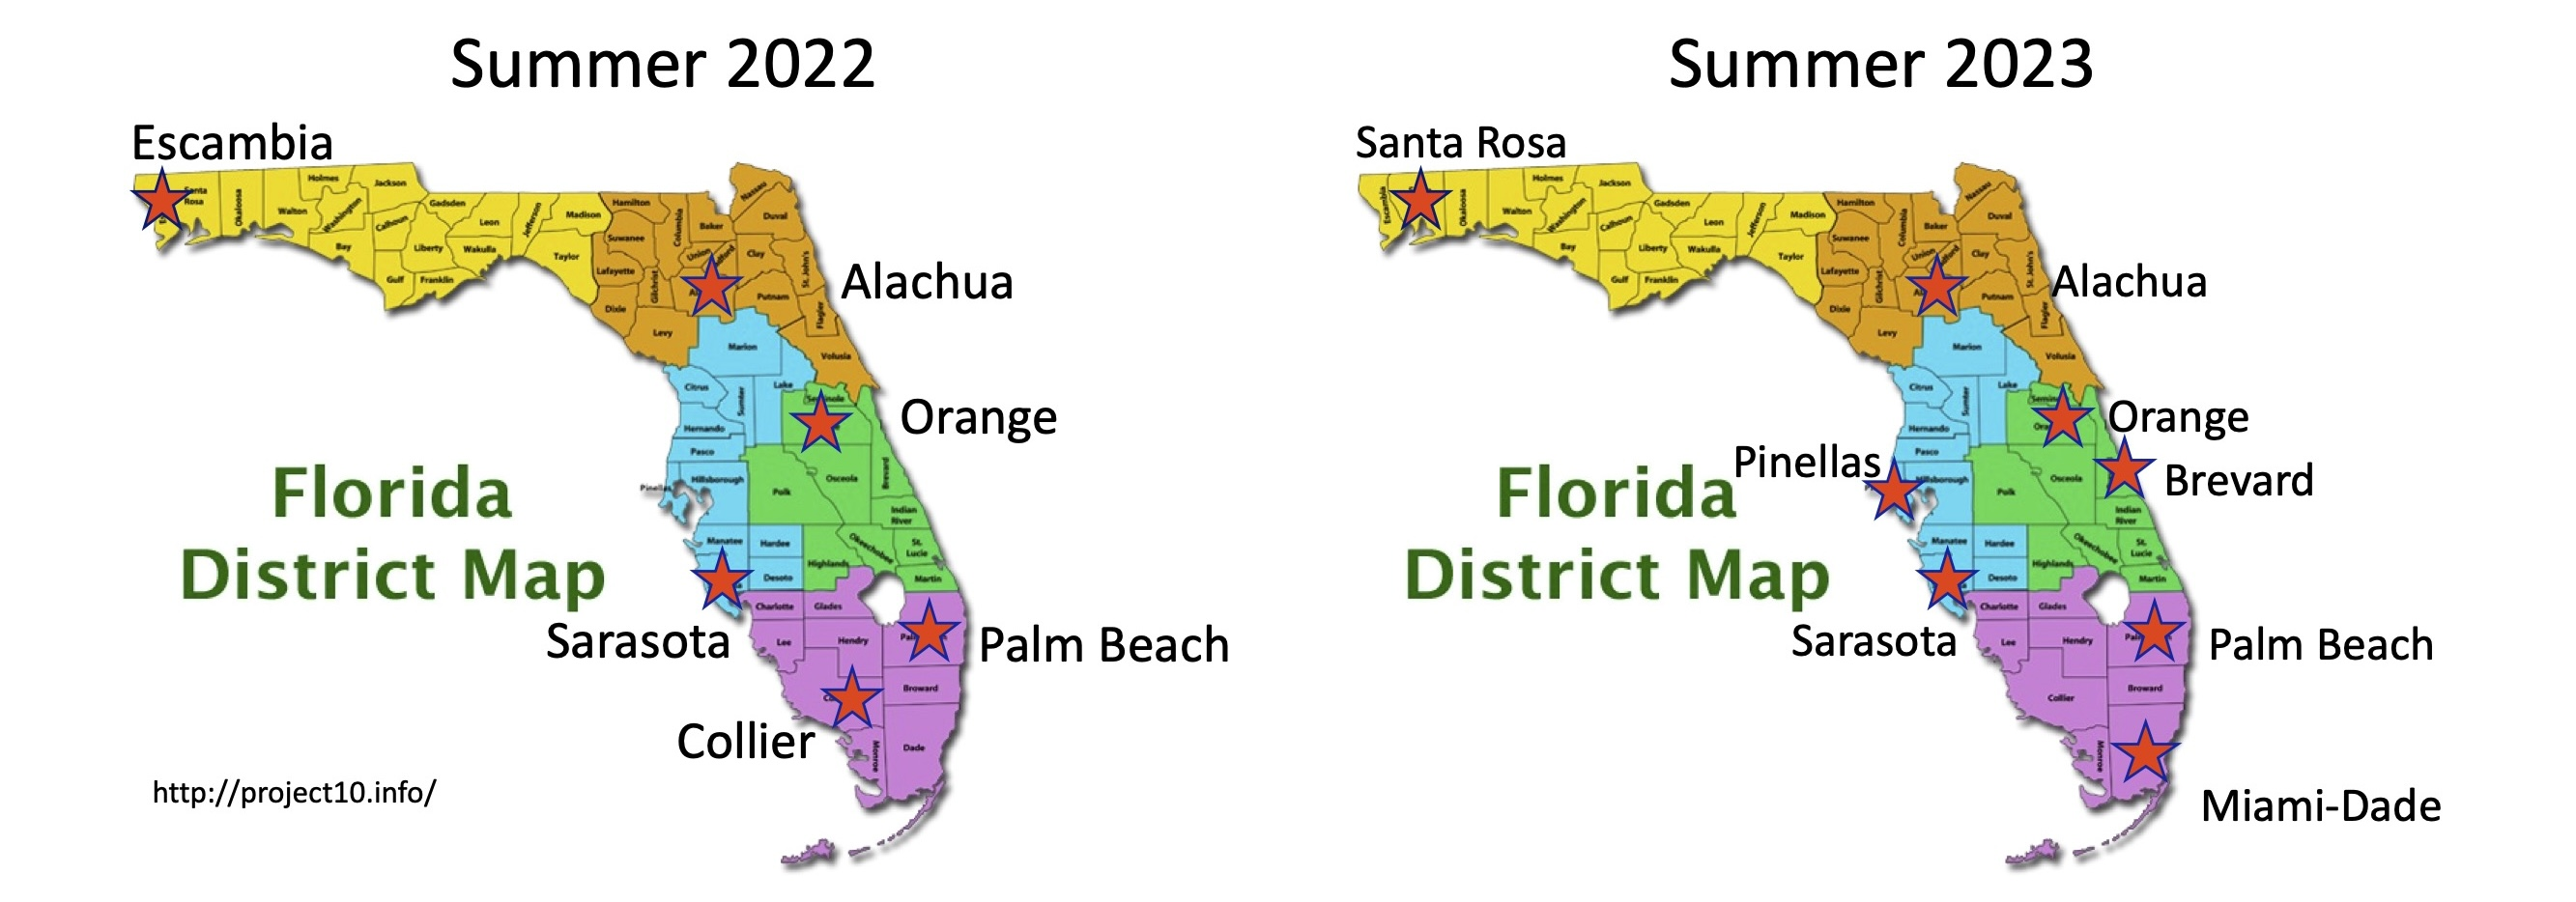
\includegraphics{Images/GGEE_23_FL District Map.jpg}
\caption{\emph{GGEE Summer Program Districts from 2022 and 2023}}
\end{figure}

\hypertarget{program-locations}{%
\subsection{Program Locations}\label{program-locations}}

The 22 program locations, schools, program levels and formats are listed
in Table 3. Of the 22 programs, 3 piloted the advanced program and the
remaining 19 were introductory levels programs to introduce students to
programming and micro:bits.

\begin{longtable}[]{@{}llll@{}}
\caption{2023 Goldberg Gator Engineering Summer Program Locations,
Programs, and Formats.}\tabularnewline
\toprule\noalign{}
School District & School/Organization Name & Program Level & Format \\
\midrule\noalign{}
\endfirsthead
\toprule\noalign{}
School District & School/Organization Name & Program Level & Format \\
\midrule\noalign{}
\endhead
\bottomrule\noalign{}
\endlastfoot
Alachua County Schools & Take Stock In Children & Advanced & 2-day,
Full \\
Brevard Public Schools & Stone Middle School & Introductory & 4-day,
Full \\
City of Rivieria Beach - Palm Beach County & Youth Empowerment Programs
& Introductory & 8-day, Half \\
Miami Dade County Public Schools & Homestead Senior High School &
Introductory & 8-day, Half \\
Miami Dade County Public Schools & North Miami Beach Senior High &
Introductory & 8-day, Half \\
Orange County Public Schools & University High School & Introductory &
4-day, Full \\
Orange County Public Schools & University High School & Advanced &
4-day, Full \\
Orange County Public Schools & University High School & Introductory &
4-day, Full \\
Orange County Public Schools & University High School & Introductory &
4-day, Full \\
Pinellas County Schools & East Lake High School & Introductory & 4-day,
Full \\
Pinellas County Schools & Lakewood High School & Introductory & 4-day,
Full \\
Santa Rosa County District Schools & Central School & Introductory &
8-day, Half \\
Santa Rosa County District Schools & Gulf Breeze High School &
Introductory & 8-day, Half \\
Santa Rosa County District Schools & Gulf Breeze High School &
Introductory & 8-day, Half \\
Santa Rosa County District Schools & Milton High School & Introductory &
8-day, Half \\
Santa Rosa County District Schools & Navarre High School & Introductory
& 8-day, Half \\
Santa Rosa County District Schools & Navarre High School & Introductory
& 8-day, Half \\
Sarasota County Schools & Booker Middle School & Introductory & 4-day,
Full \\
Sarasota County Schools & Booker Middle School & Advanced & 4-day,
Full \\
School District of Palm Beach County & Bear Lakes Middle School &
Introductory & 8-day, Half \\
School District of Palm Beach County & Carver Middle School &
Introductory & 8-day, Half \\
School District of Palm Beach County & Lake Shore Middle School &
Introductory & 8-day, Half \\
\end{longtable}

\hypertarget{program-calendar}{%
\subsection{Program Calendar}\label{program-calendar}}

Each program was given the option to host a session over 1-2 weeks from
June 5th through July 24th, 2023. Many programs overlapped during the
9-week window as shown in
\textbf{\emph{\protect\hyperlink{appendix-1-summer-program-calendar}{Appendix
1: Summer Program Calendar}}}. Programs are color coded by district and
locations with more than one session were given a number at the end,
such as Orange Intro 1. Sessions that were held across two weeks are
listed in both weeks. The least popular week was July 3rd-7th with one
session running, likely due to the fourth of July holiday. The most
popular week to host a summer program was June 19th-22nd with a total of
nine sessions.

\hypertarget{program-layouts}{%
\section{Program Layouts}\label{program-layouts}}

The GGEE summer programs were designed to provide options that best fit
with school district's summer schedules and existing summer programs. To
better accommodate and support our programs, we structured them to run
on 4-day schedules for either 4 full-days for 7-8 hour days or 8
half-days for 4-5 hour days. When working with schools we founds that
some ran for an entire day, some were open for half of a day, and almost
all locations were closed on Fridays.

\hypertarget{introductory-programs}{%
\subsection{Introductory Programs}\label{introductory-programs}}

The Introductory Program design allowed students with varying skill
levels to participate. The program can be run in 4-day, full-day or
8-day, half-day programs. A roadmap, Figure 2, was developed to walk
through the program by day. The goals for the first day of the program
were to introduce the team, goals for the program, collaborative
learning strategies, and Micro:bit programming basics using no-code and
low-code activities. The program then introduced students to their first
design-based activity where they were challenged with designing a
Micro:bit Pet for their partner using the Stanford design cycle:
Empathize, Define, Ideate, Prototype, Test. While designing the Pet,
students had to learn to wire and program external sensors and motors to
the Micro:bit to create additional features for pets. The remainder of
the program focused on a technical design challenge where student groups
worked together in a project team to design a solution for one of three
challenges: temperature regulation in a greenhouse, an acceleration
indicator for a new driver, and a remotely activated stoplight for first
responders. Together, they stepped through the design cycle to develop
solutions to these challenges like many engineers and scientists. They
also developed teamwork and program management skills during the
technical design challenge.

\begin{figure}
\centering
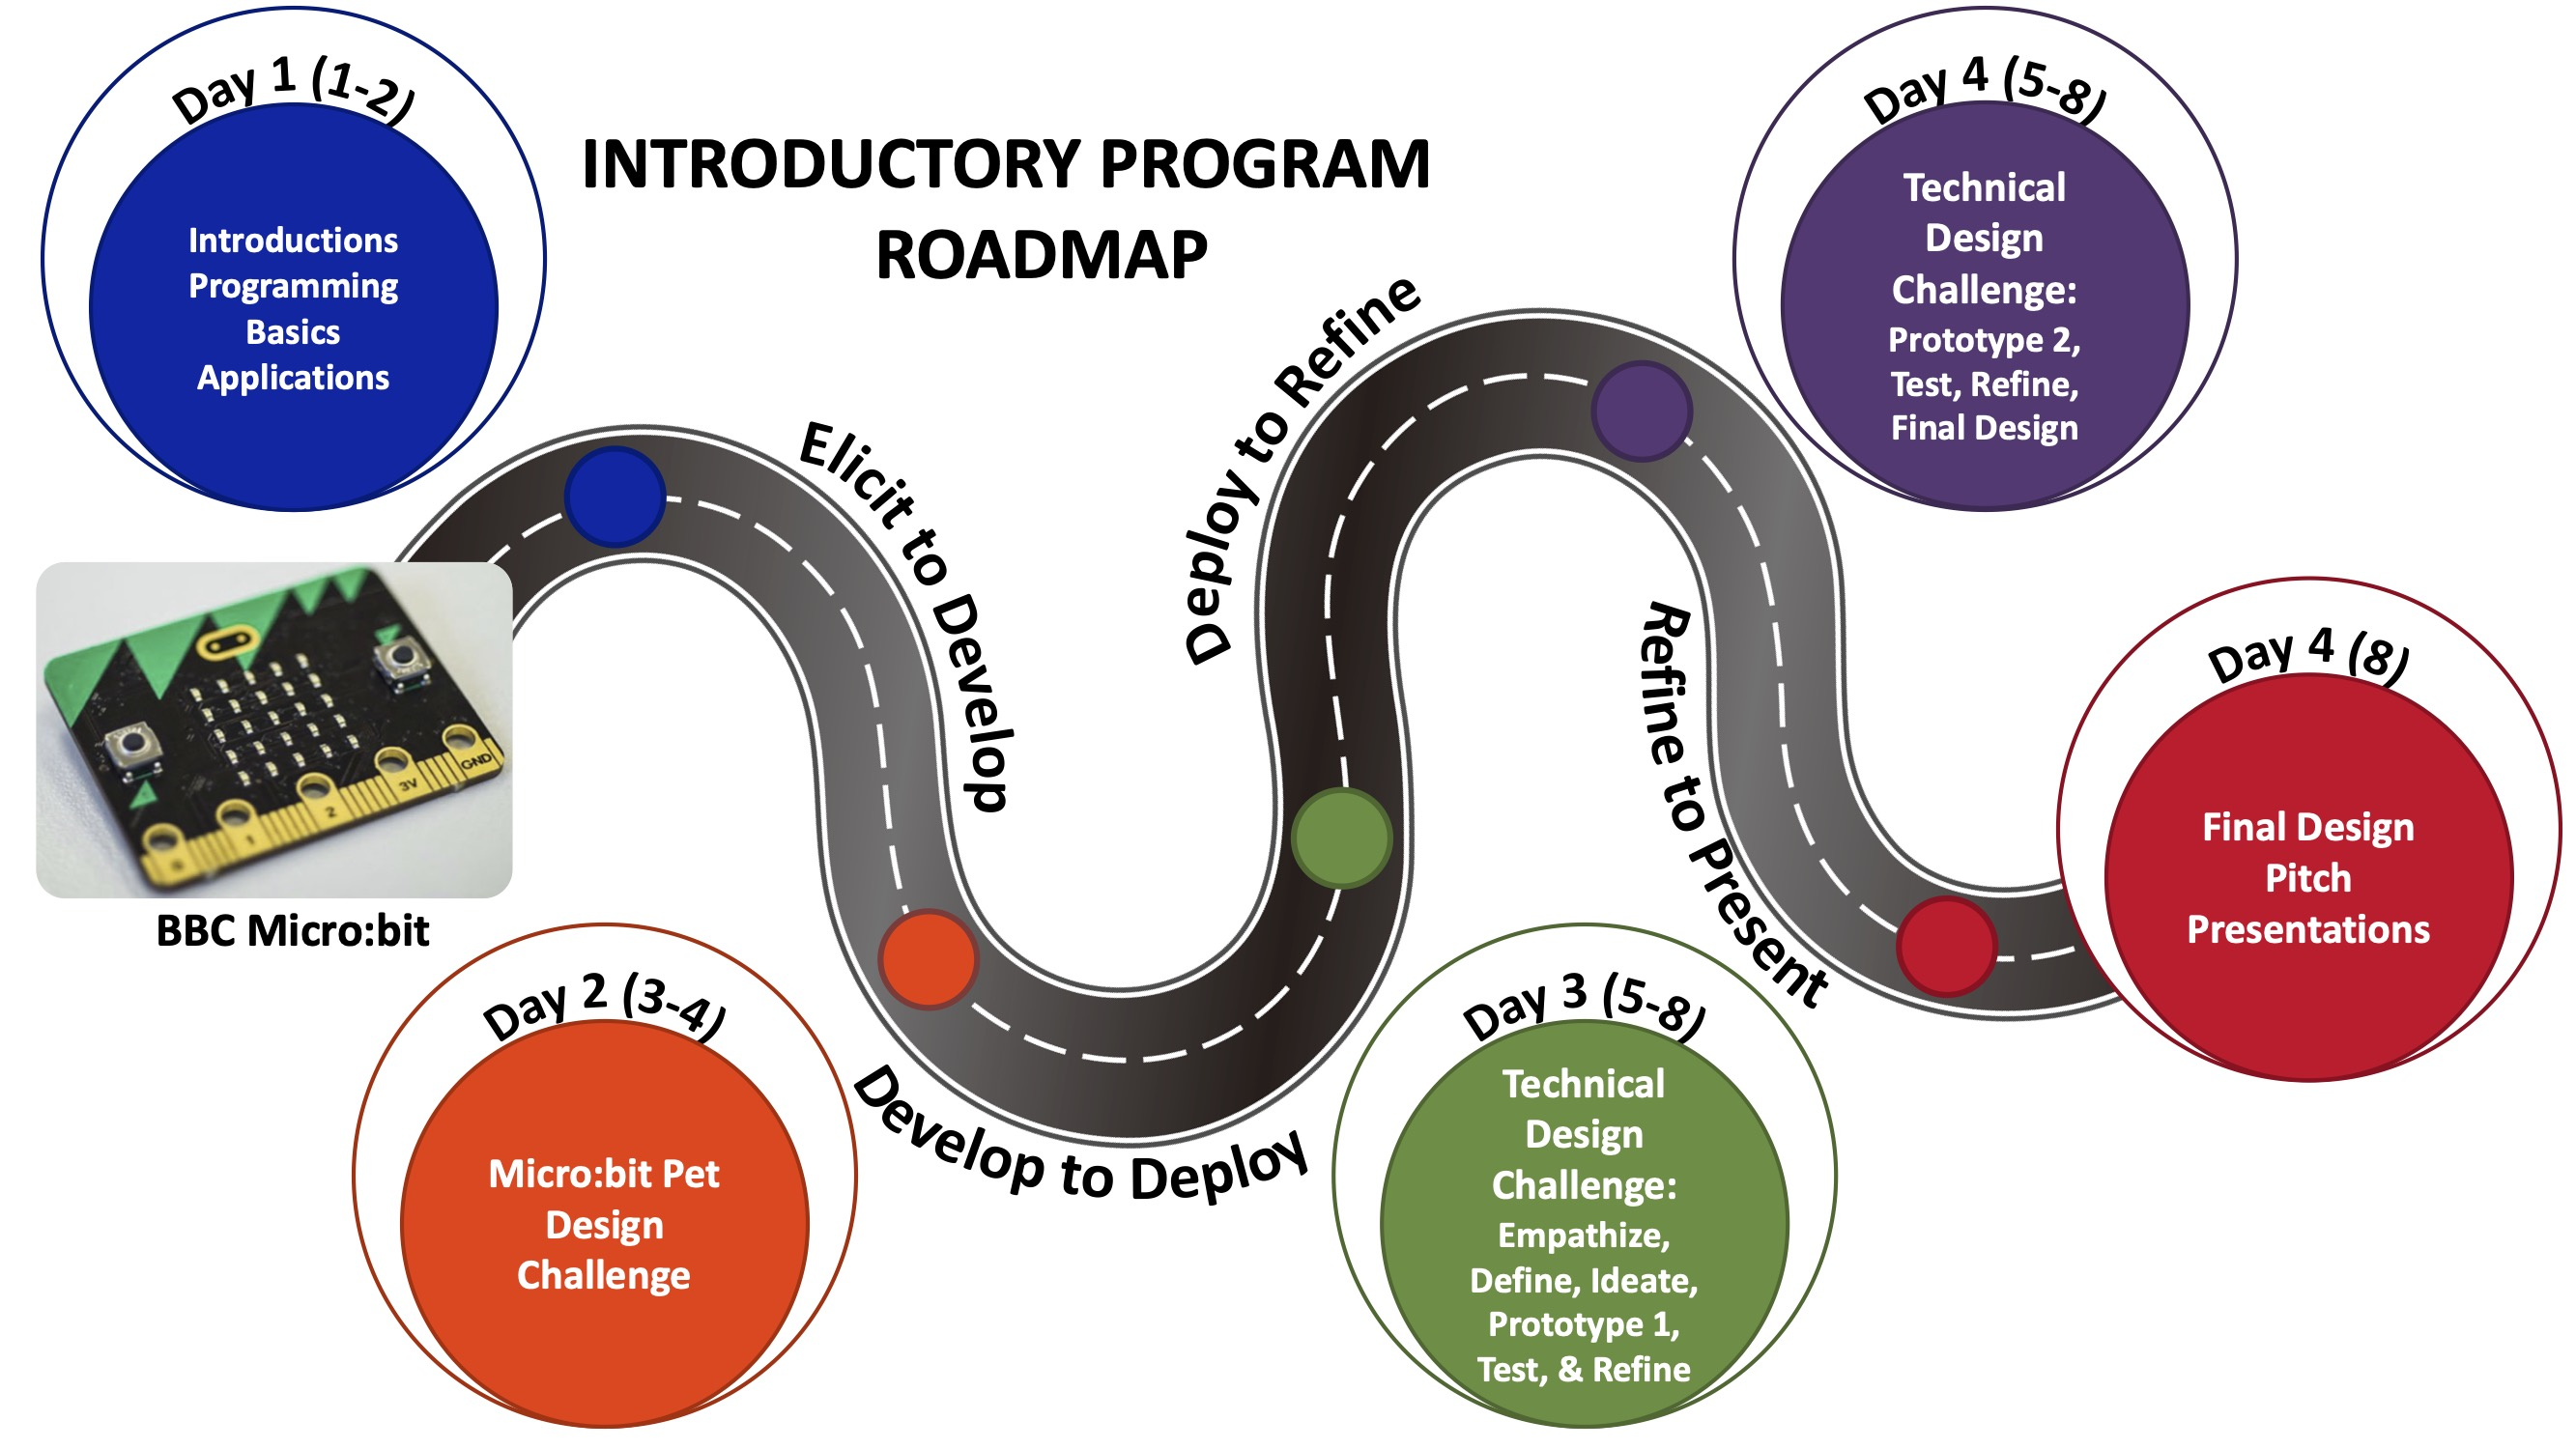
\includegraphics[width=0.65\textwidth,height=\textheight]{Images/GGEE_23_intro_roadmap.jpg}
\caption{\emph{Introductory Program Roadmap}}
\end{figure}

\hypertarget{advanced-programs}{%
\subsection{Advanced Programs}\label{advanced-programs}}

The Advanced Program was formatted as 4 day program in all the pilot
schools, Figure 3. Students were first introduced to the basic concepts
of artificial intelligence and then machine learning. The day was
concluded with an introduction to programming in
\textbf{\emph{\href{https://scratch.mit.edu/}{Scratch}}} to prepare for
the following day when students were introduced to Image-based and
Test-based machine learning models from
\textbf{\emph{\href{https://machinelearningforkids.co.uk/}{Machine
Learning for Kids}}}. Students develop and train a image-based machine
learning model that analyzes the color characteristics of different
types of Pokémon. They then trained a text-based machine learning model
to design a smart classroom that had electronic devices that power on or
off using a variety of written commands. On the third day, students use
their micro:bit programming skills from last summer program to program a
micro:bit to identify different types of gestures. During this activity,
students built their own sets of training data using the micro:bits.
Students program gestures together as a class and a number of gestures
on their own. The machine learning models were trained using a decision
tree constructed in Python and hosted in a Juypter Notebook on
\textbf{\emph{\href{https://nanohub.org/}{NanoHub}}}. The model was
loaded onto the micro:bit giving it the ability to identify gestures
based on the training data provided. To round out the program, students
were introduced to Neural Networks. The activity walked them through the
various types of machine learning models from decision trees to more
complex neural networks. Students learned about the multiple layers in a
neural network and the processes that each of those layer serve. The
following activity had students develop and train a neural network to
identify images of numbers. Students manipulated the number of nodes and
studied the effect on the outcame and weights in identifying each
number. This activity concluded the program.

\begin{figure}
\centering
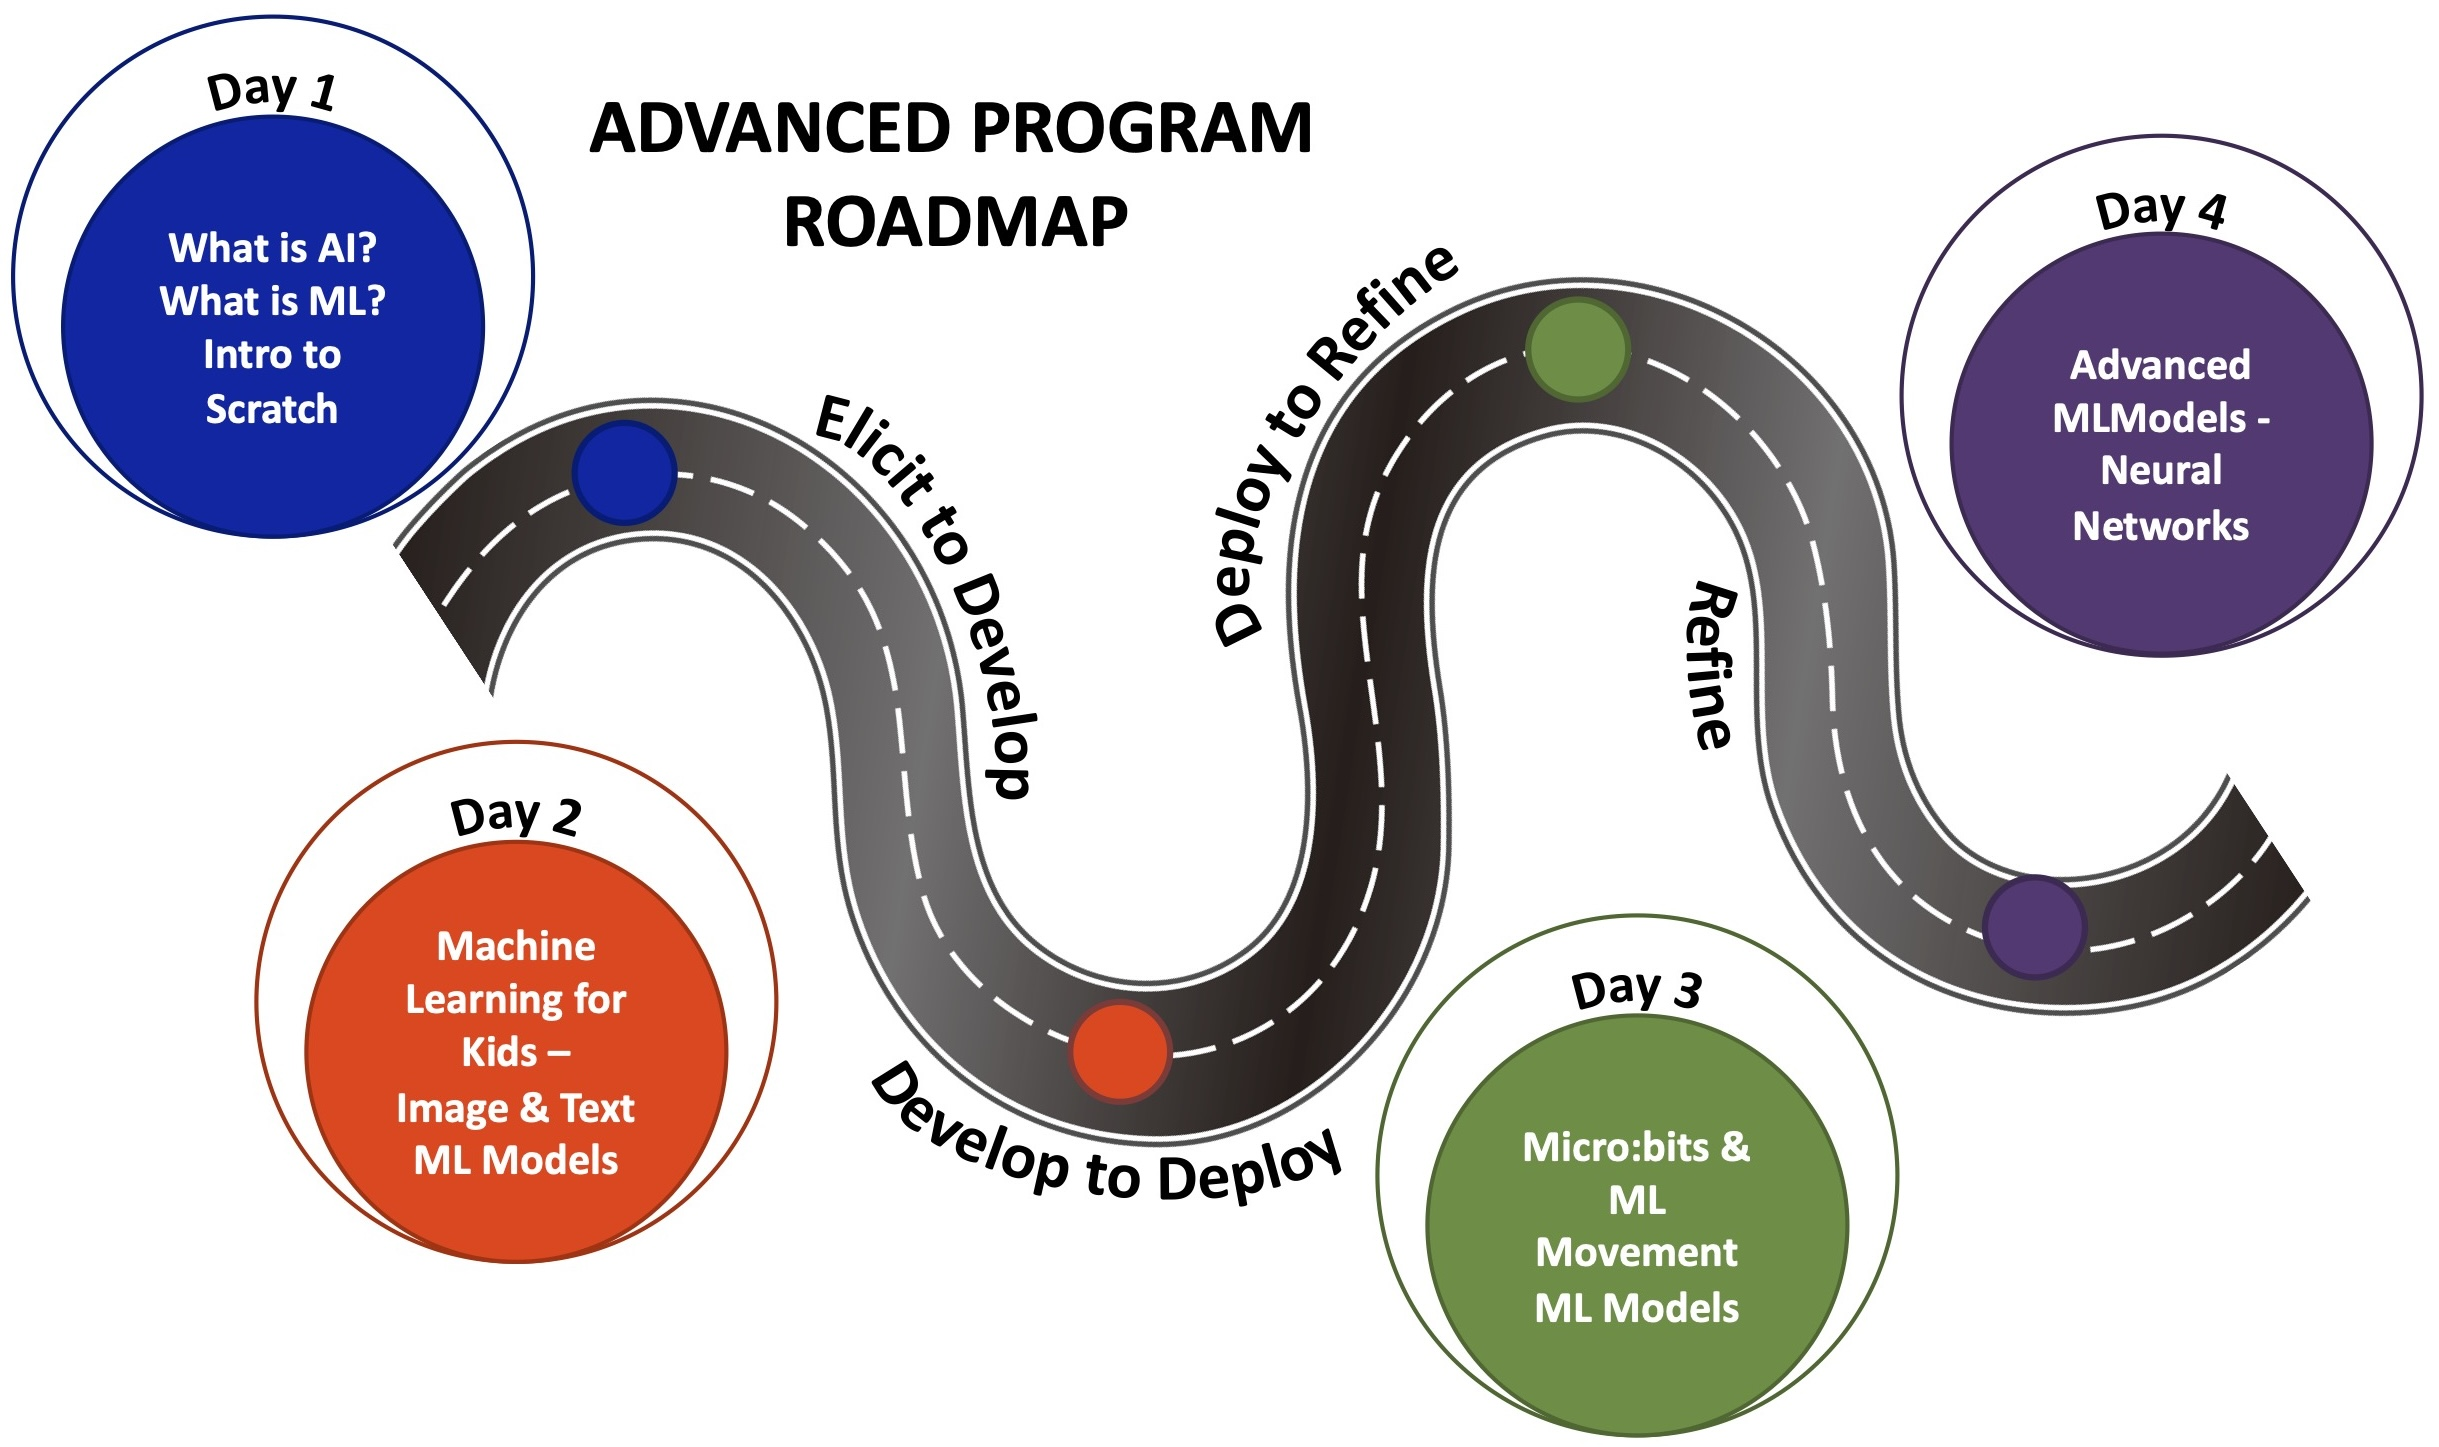
\includegraphics[width=0.65\textwidth,height=\textheight]{Images/GGEE_23_Adv_roadmap.jpg}
\caption{\emph{Advanced Program Roadmap}}
\end{figure}

\hypertarget{student-enrollment-demographics}{%
\section{Student Enrollment \&
Demographics}\label{student-enrollment-demographics}}

\hypertarget{enrollment}{%
\subsection{Enrollment}\label{enrollment}}

There were a total of 713 student registrations completed for the GGEE
2023 summer programs. Table 4 displays how many registrations were
completed for each distrcit as well as how many programs were held in
the location.

\begin{longtable}[]{@{}lcc@{}}
\caption{Total number of registrations by district before enrollment
limits and wait lists.}\tabularnewline
\toprule\noalign{}
District & Number of Students & Number of Programs \\
\midrule\noalign{}
\endfirsthead
\toprule\noalign{}
District & Number of Students & Number of Programs \\
\midrule\noalign{}
\endhead
\bottomrule\noalign{}
\endlastfoot
Alachua County & 20 & 1 \\
Brevard County & 23 & 1 \\
Miami-Dade County & 90 & 2 \\
Orange County & 90 & 4 \\
Palm Beach County & 88 & 4 \\
Pinellas County & 40 & 2 \\
Santa Rosa County & 336 & 6 \\
Sarasota County & 26 & 2 \\
\end{longtable}

Recruitment of students for the GGEE summer programs were managed by the
districts and schools while the enrollment registration process was
managed by the EQuIPD team through a Qualtrics survey. Programs were
limited to 25 student registrants with the expectation that around 20
students would attend the program. When the registration limit was met
for a program, the option for the program was marked as ``FULL'' and
parents were set a wait list notice email, instead of the confirmation
email regularly sent. Students would move from the wait list to the main
registration when parents would withdraw their students from the program
prior to the start of the program.

Parents continued to register their children for the program and join
the wait list. Session registrations averaged around 33 students per
session. The highest number of registrations being 113 students for the
Santa Rosa County, Milton High School Introductory program from July
10-13 + 17-20.

\hypertarget{attendance}{%
\subsection{Attendance}\label{attendance}}

After limiting the program to 25 students, actual attendance of the
programs averaged around 15 students per program with 319 students
participating in a 2023 Goldberg Gator Engineering Explorer Summer
Program, Figure 4. The districts with the largest number of student
participants were as follows: Santa Rosa County - 111 students in 6
sessions, Palm Beach County - 56 students in 4 sessions, and Orange
County - 55 students in 4 sessions.

While most programs reached the 25 student registration limit for the
summer program, there were less students actually attended the programs
due to falling ill, unexpected family travel, or changes in plans
without notifying our program. Students were moved up on the wait list
up until the first day of the program. Once the program started, no
students were moved from the wait list to ensure the program would meet
youth compliance adult to student ratios and to prevent students falling
behind after missing the essential concepts covered during day one.

There were 284 students that participated in the 19 Introductory GGEE
summer program sessions and 35 students that participated in the 3
Advanced GGEE summer program sessions. The breakdown of student
attendance by program level is shown in Figure 5. The highest number of
students in attendance for a program was 24 students at Santa Rosa
County, Navarre High School Introductory Program from June 5-8 + 12-15.
The lowest attendance was 8 students participating in the Orange County,
University High School Advanced Program from June 5-8.

When looking at the distribution of students in the introductory
programs the large percentage from Santa Rosa County aligns with the
number of sessions they hosted, Figure 5. Santa Rosa held the most
sessions in a given district providing the most opportunities for
students to participate in the program. Nearly half of the students in
the advanced programs were from Orange County. During the previous pilot
year Orange county held 3 introductory sessions providing a larger base
of students to recruit to participate in the advanced program.

\begin{figure}
\centering
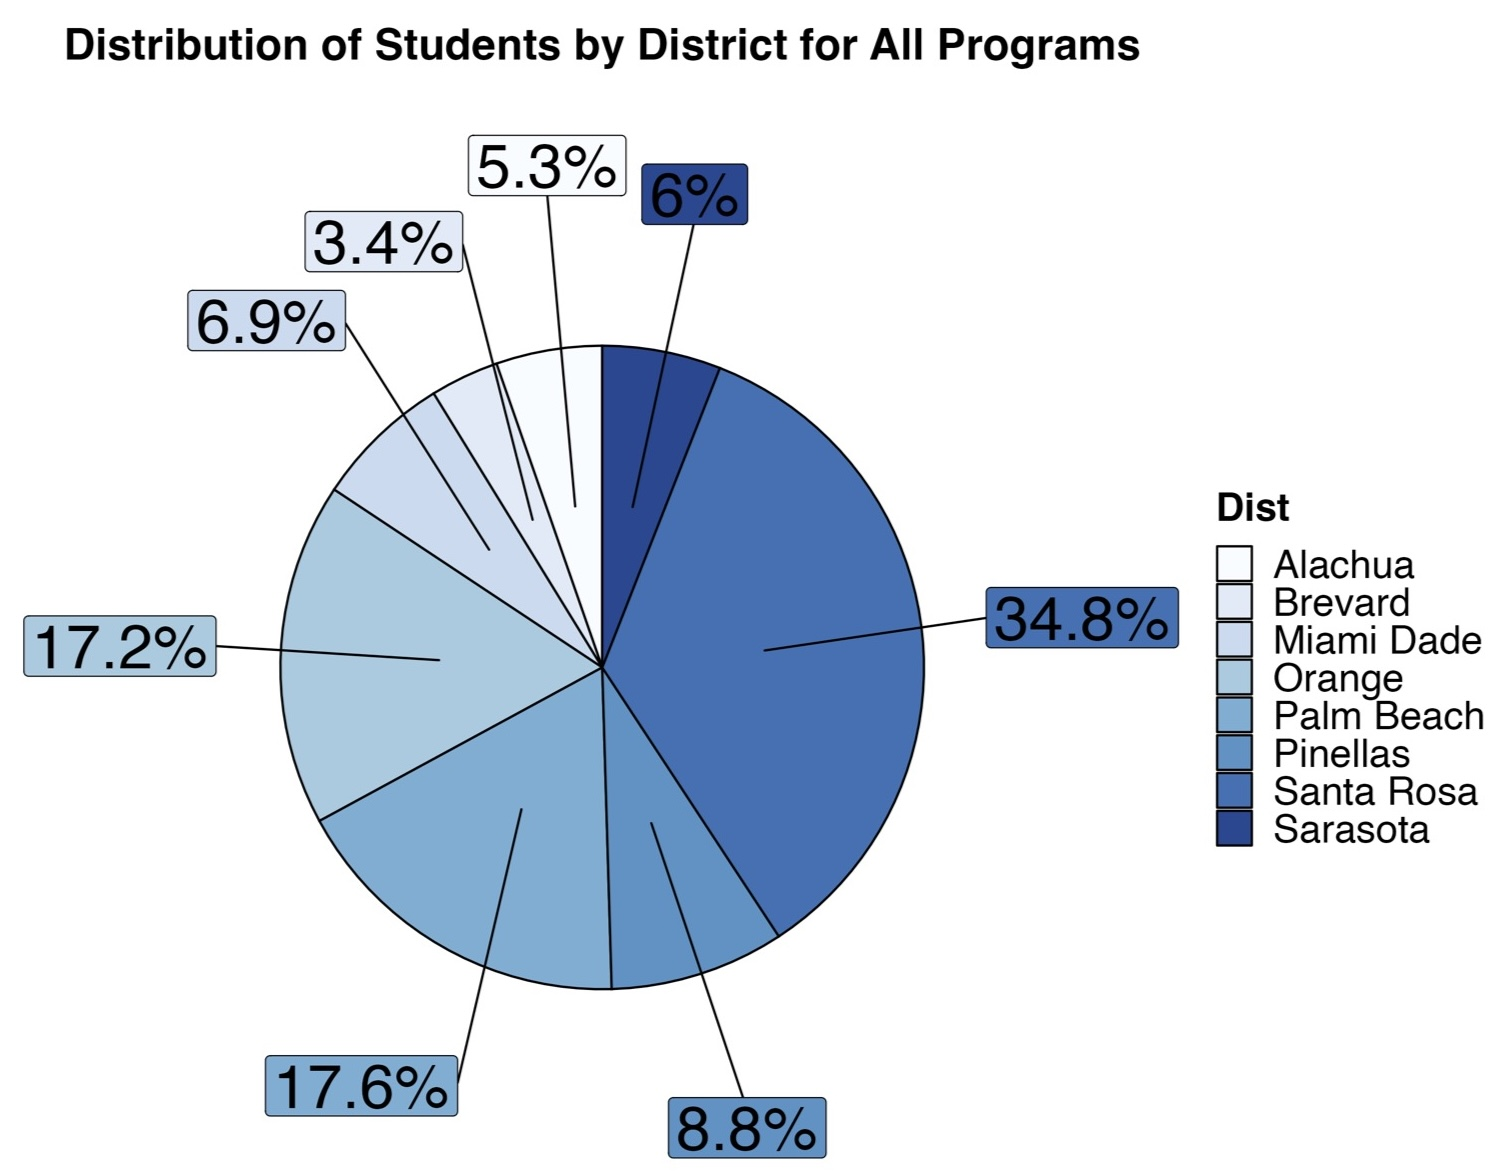
\includegraphics[width=0.5\textwidth,height=\textheight]{Graphs/Report/GGEE_23_District_All.jpg}
\caption{\emph{The distribution of students by district for both
introductory and advanced Goldberg Gator Engineering Explorer Summer
Programs (n=319)}}
\end{figure}

\begin{figure}
\centering
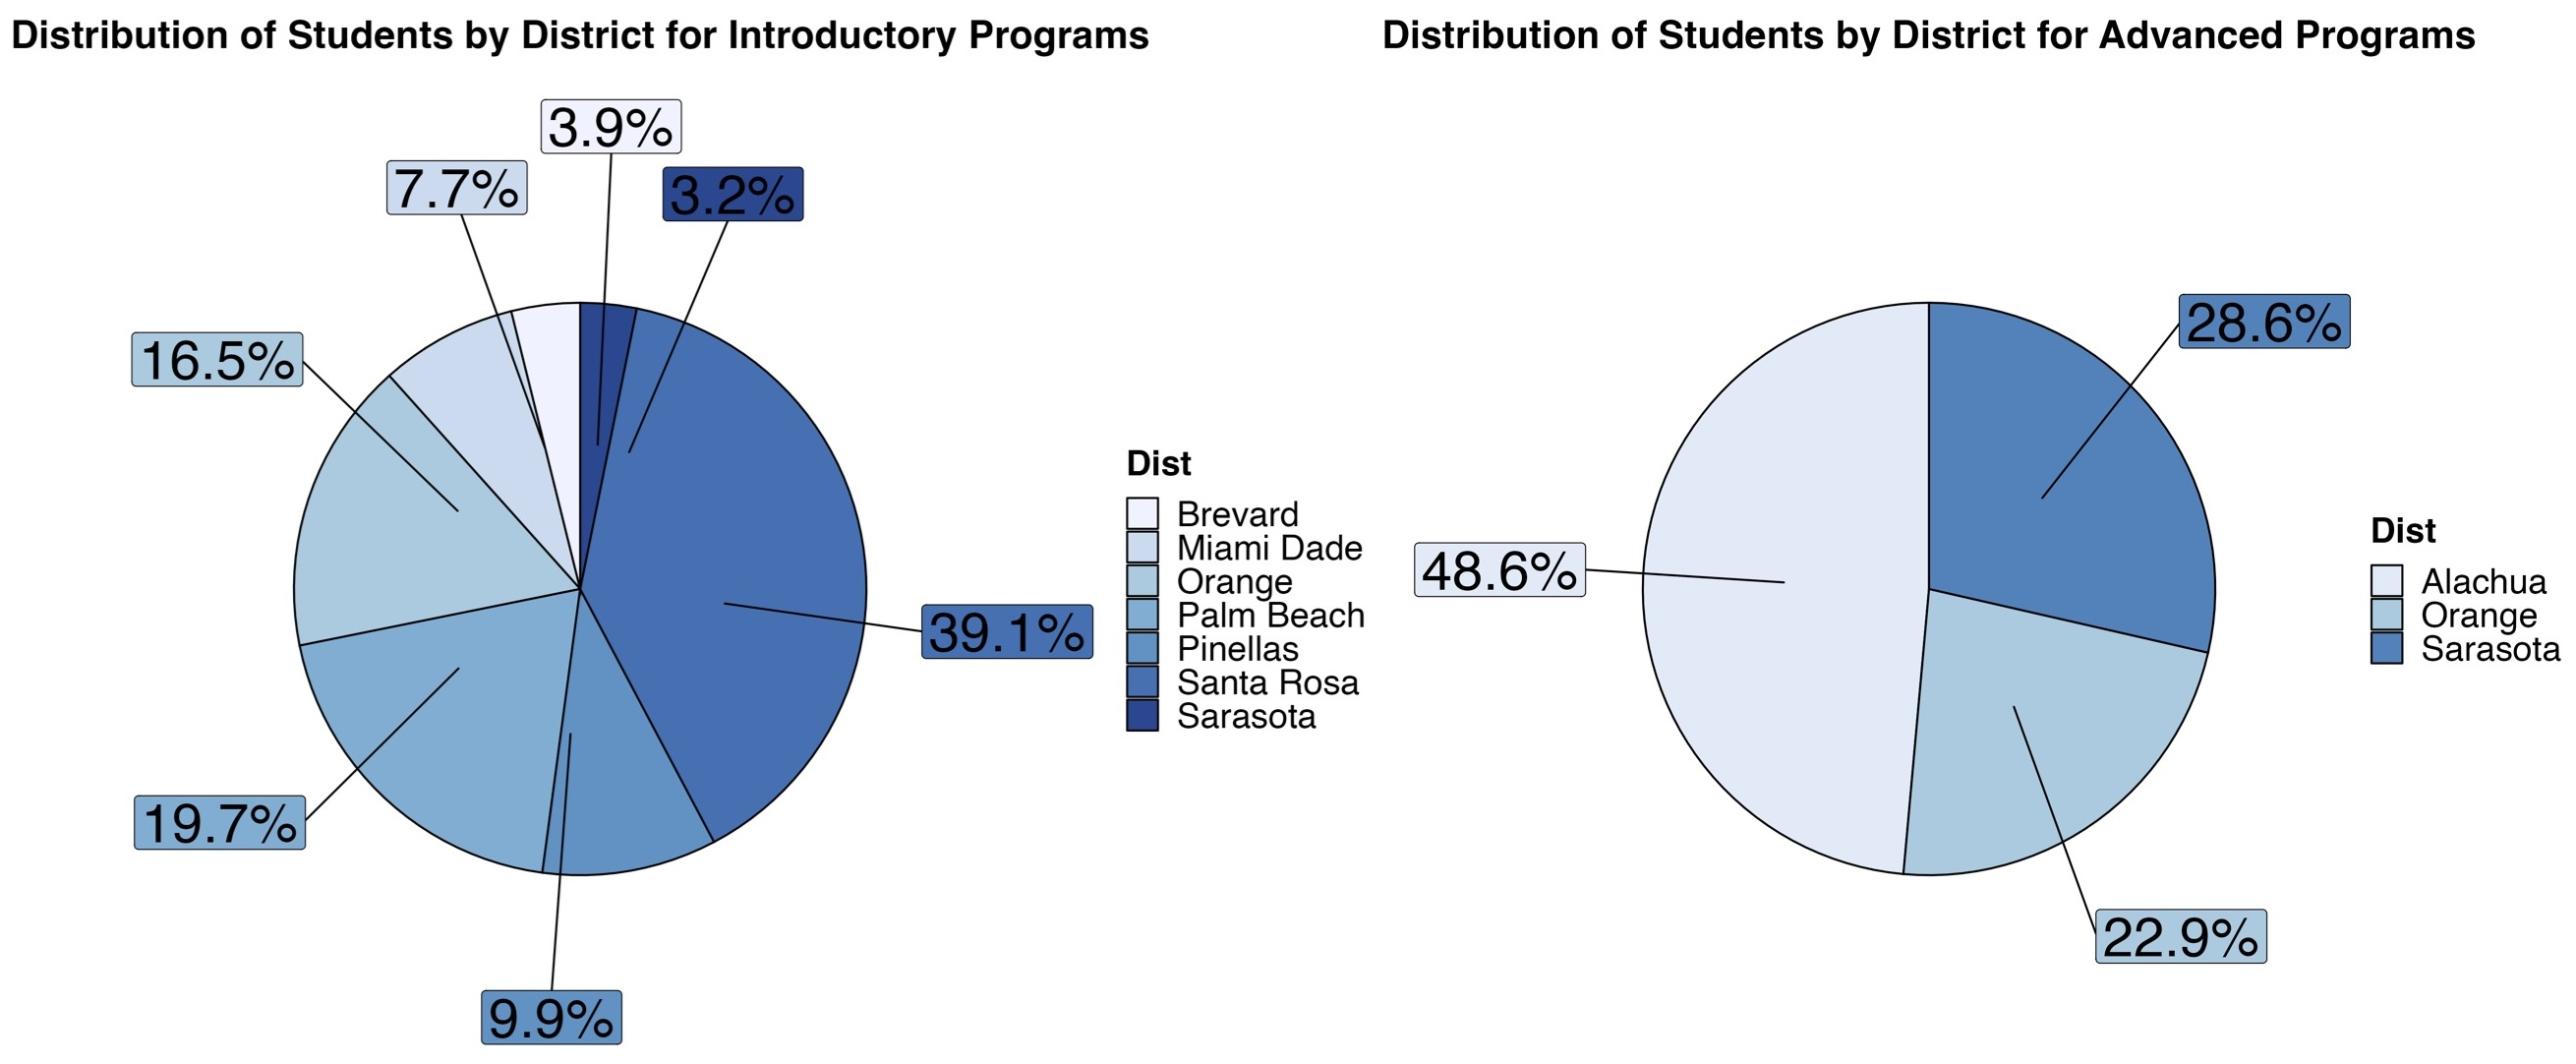
\includegraphics[width=0.9\textwidth,height=\textheight]{Graphs/Report/GGEE_23_District_IA.jpg}
\caption{\emph{The distribution of students by district for the
introductory (left, n=284) and advanced (right,n=35) Goldberg Gator
Engineering Explorer Summer Programs}}
\end{figure}

\hypertarget{student-demographics}{%
\subsection{Student Demographics}\label{student-demographics}}

Student demographics were collected from students that participated in
the research study by permission of their parents. The results for
student demographics were taken from the Pre-Survey that students
completed at the start of the program. To ensure consistency in results,
surveys that were taken after the first day of the respective program
were removed from analysis in addition to responses that were missing a
critical demographic response such as age, grade, race/ethnicity, or
gender. Students participating in Alachua county's Take Stock in
Children advanced program were not surveyed or interviewed because the
session was modified to two days unlike the other programs with full 4
or 8 day experiences. There were a total of 204 Pre-survey student
responses that were analyzed for the GGEE Summer programs, 194 students
participated in an introductory level program and 10 participated in an
advanced level program.

\hypertarget{age-and-grade-level}{%
\subsubsection{Age and Grade Level}\label{age-and-grade-level}}

The GGEE summer programs were targeted toward rising 6th to 10th
graders. The introductory programs were open to rising 6th through 9th
graders while the advanced programs were open to rising 7th to 10th
graders to include the older students that participated in the 2022 GGEE
programs and returned for a second year. This range of grade levels
invited students from the ages of 10 to 16 to participate in the
program. The distribution of ages and grade levels participating in all
GGEE summer programs are shown in Figure 6. Over 50\% of students
participating in the program are between the ages of 12 and 13 and in
either 7th or 8th grade.

\begin{figure}
\centering
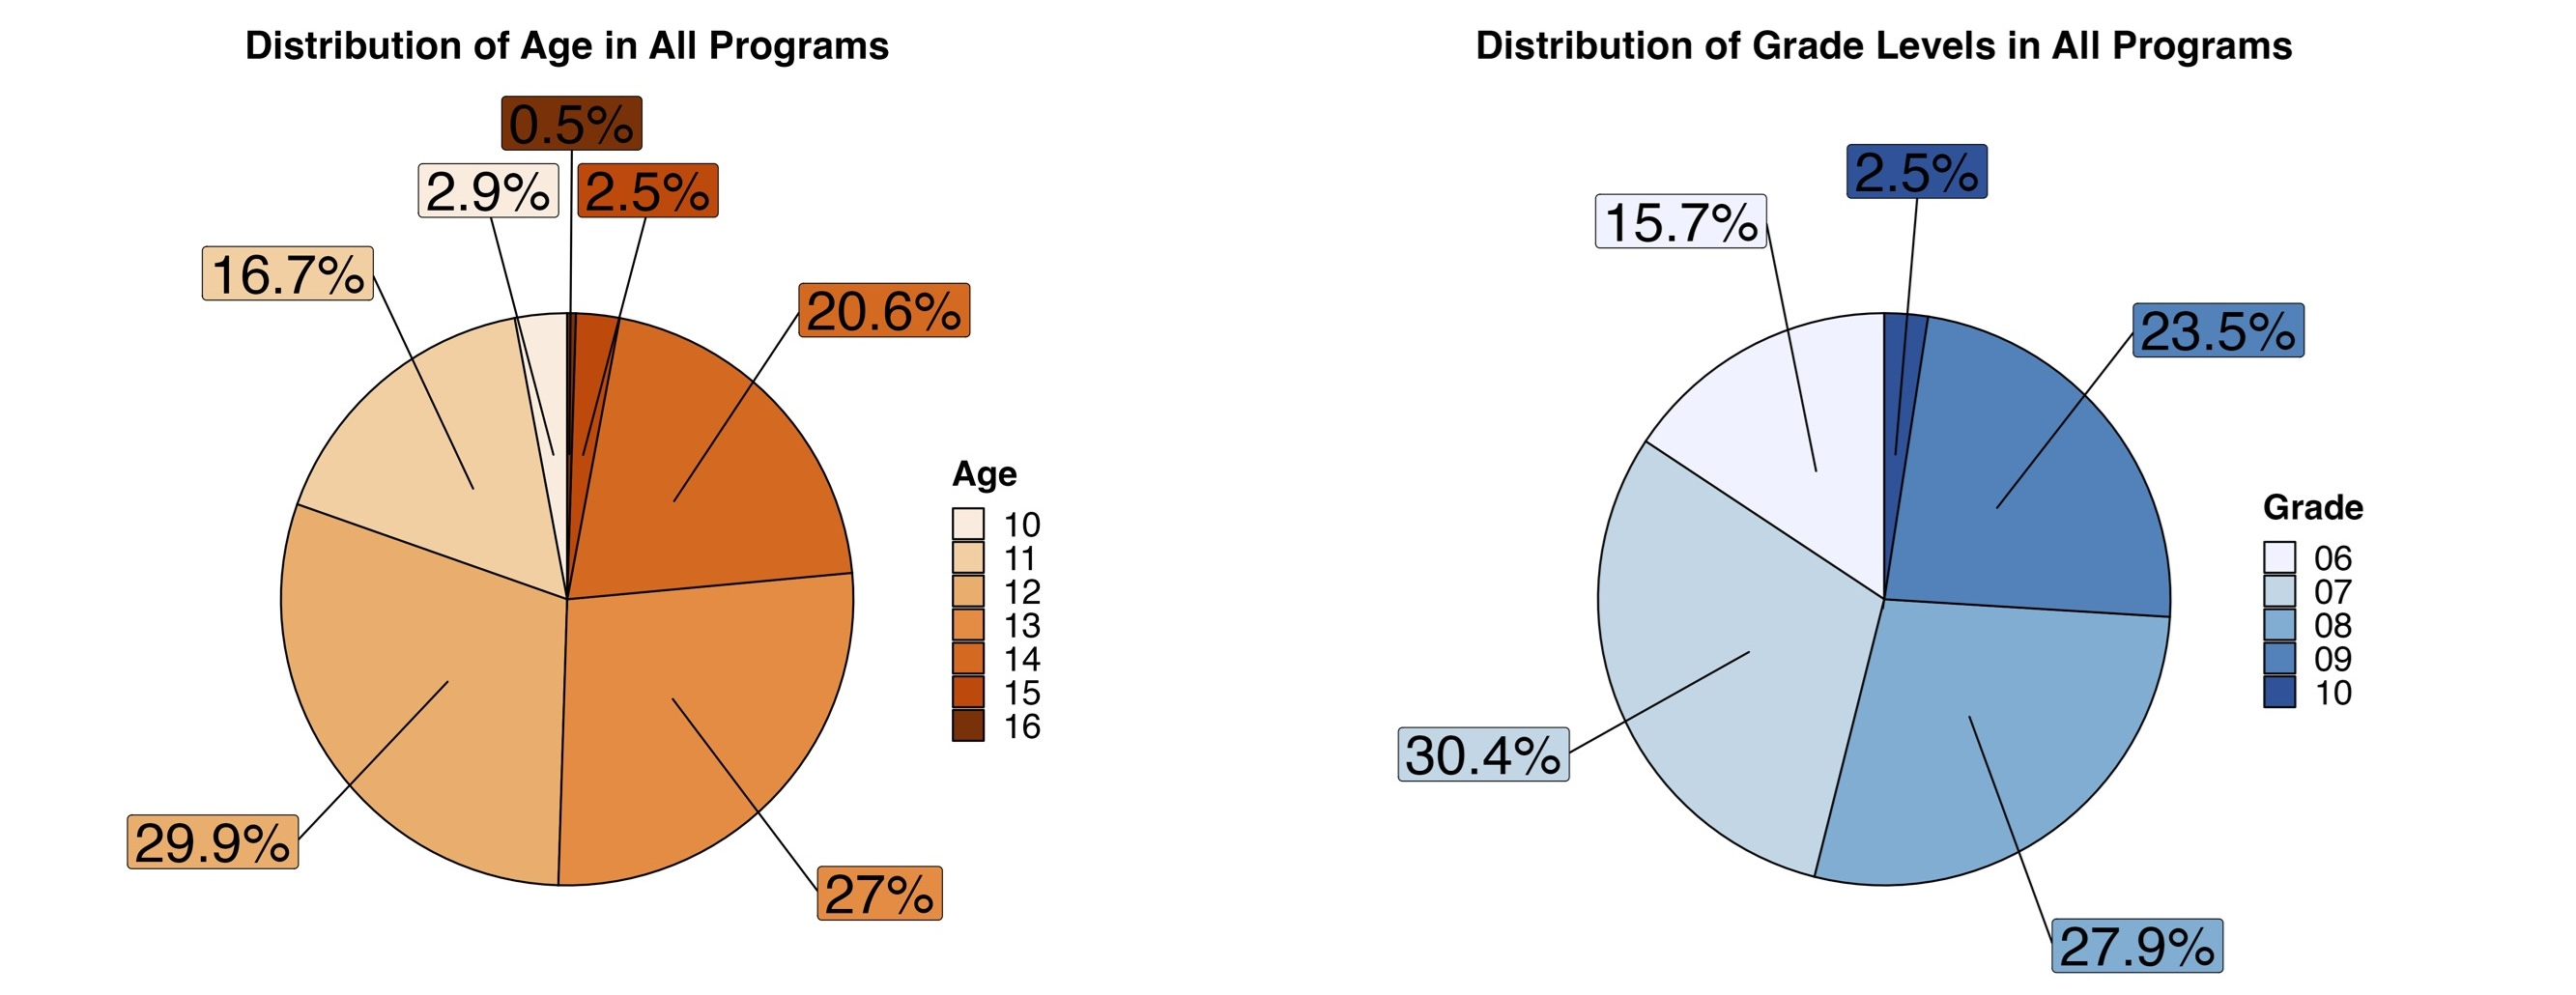
\includegraphics[width=0.8\textwidth,height=\textheight]{Graphs/Report/GGEE_23_AgeGrade_All.jpg}
\caption{\emph{The distribution of student ages (left) and student grade
levels (right) for both introductory and advanced Goldberg Gator
Engineering Explorer Summer Programs (n=204).}}
\end{figure}

When looking at the distribution of age in the introductory programs,
Figure 7, left, we see that students from ages 10-16 are participating
in the program. This is likely due to parents registering younger or
older siblings into the program to participate together. In the
introductory programs more than 50\% of students were within the target
age range of 12-13 years old and going into 7th or 8th grade. When
looking at the advanced program age distributions, Figure 7, right,
students are mainly 13 years old and equally going into 8th or 9th
grade. Since advanced program students were required to have
participated in the previous pilot year, age and grade levels were
anticipated to be higher than the introductory programs.

\begin{figure}
\centering
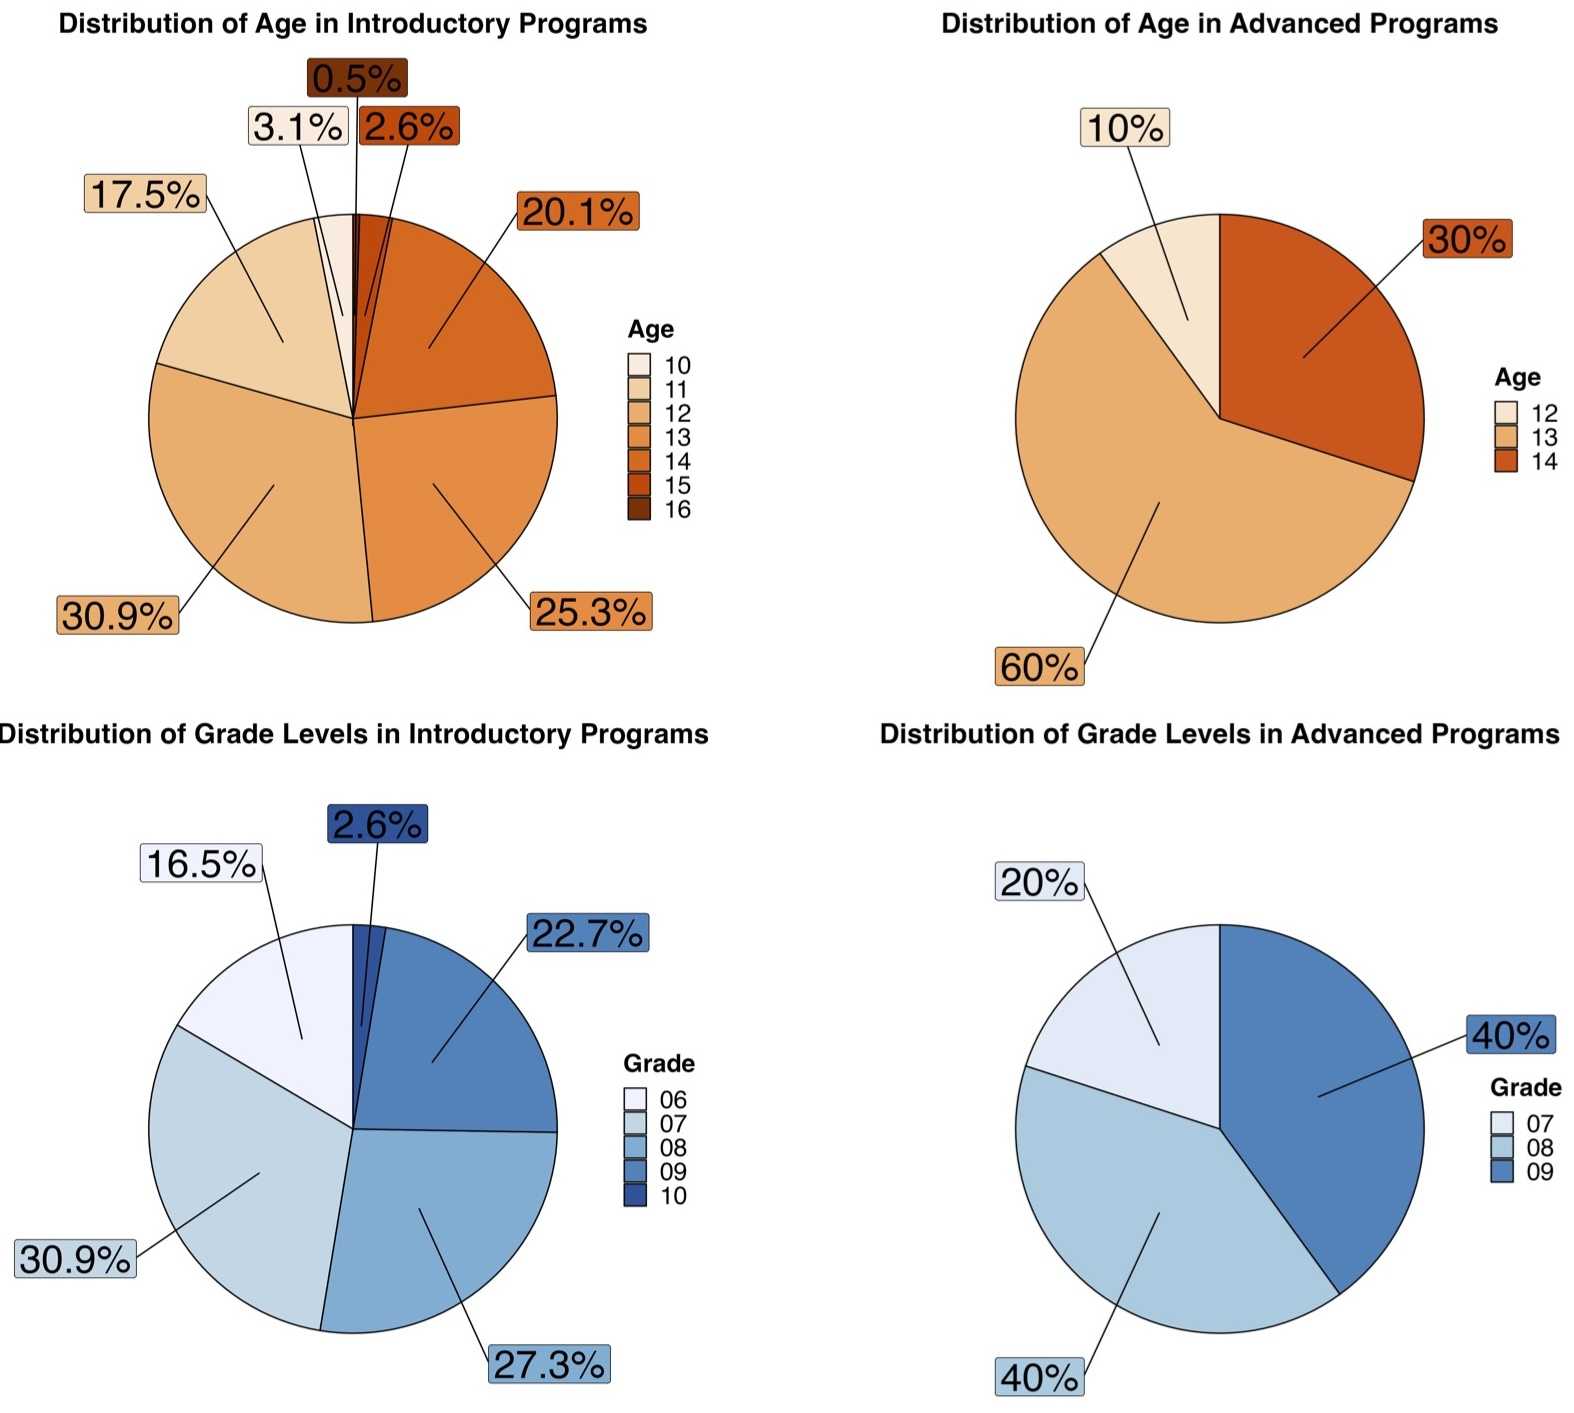
\includegraphics[width=0.85\textwidth,height=\textheight]{Graphs/Report/GGEE_23_AgeGrade_IA.jpg}
\caption{\emph{The distribution of students age and grade level for
introductory programs (left, n=194) and student age and grade level for
advanced programs (right, n=10).}}
\end{figure}

\hypertarget{gender}{%
\subsubsection{Gender}\label{gender}}

Gender demographics were collected in the pre-survey. Students were
given the following options to select from: Male, Female, Prefer to Self
Describe, and Prefer Not to Say. The Prefer to Self Describe option gave
students the chance to write in their response. The distribution of
student participant gender for all GGEE programs is shown in Figure 8.

Majority of the students participating in the research study were male,
145 students. There were 49 female students across each program. There
were 6 students who opted not to disclose their gender and 4 students
that preferred to self-describe. Of the students that self-described, 1
student left their response blank, 1 student described themselves as a
``girl'', 1 student described themselves as a ``male'', and 1 student
described themselves as a type of vehicle, which is assumed to be a part
of a joke.

\begin{figure}
\centering
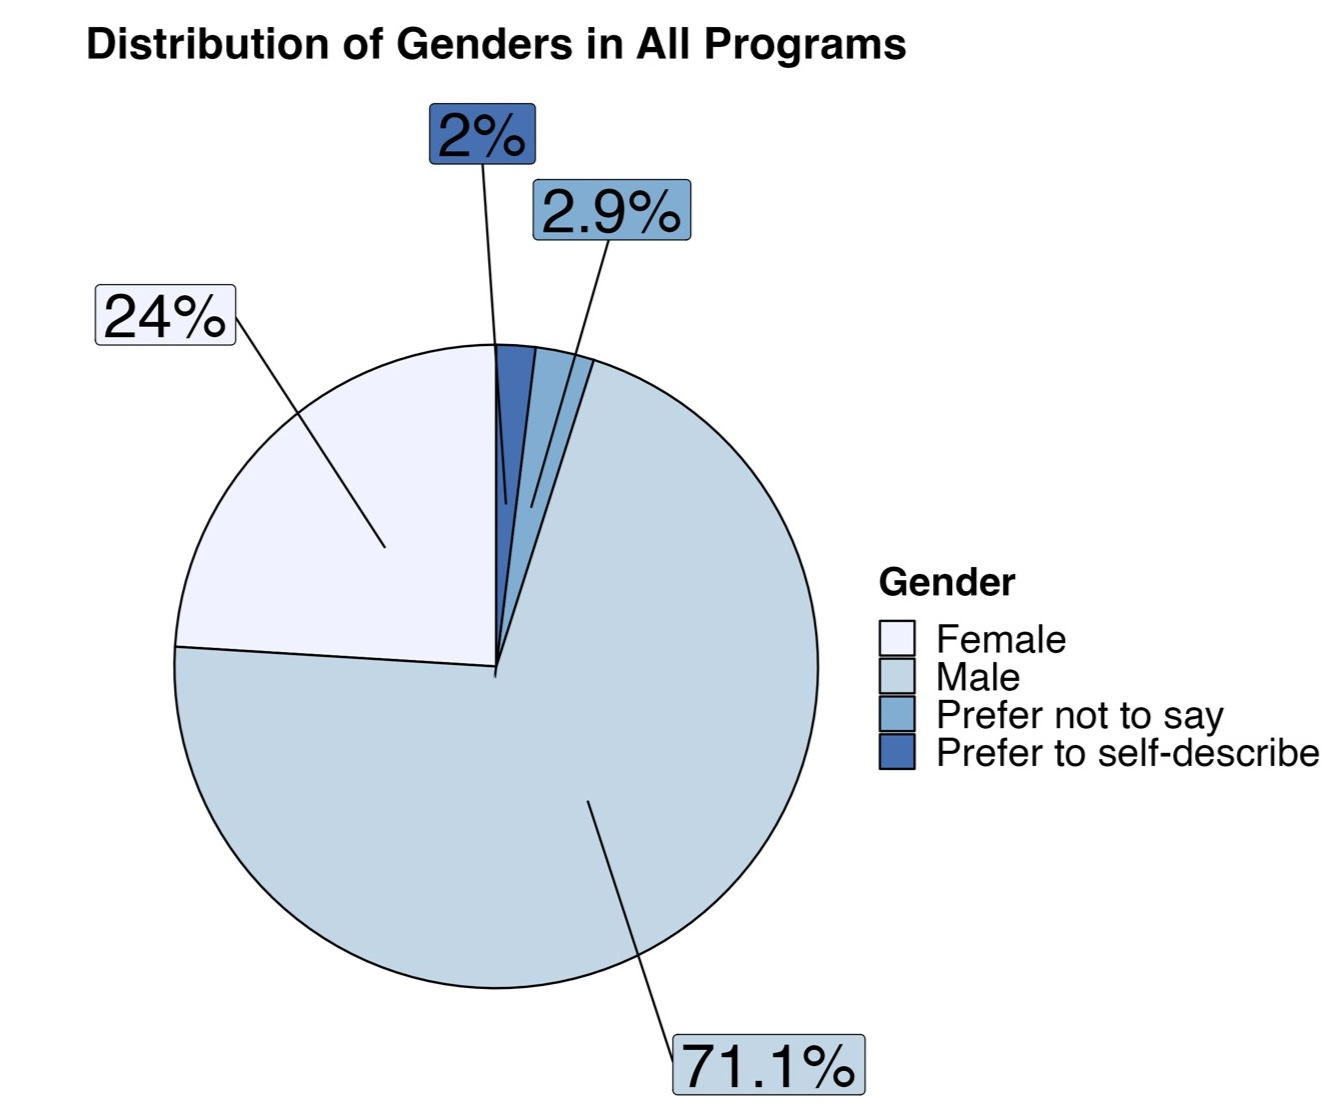
\includegraphics[width=0.5\textwidth,height=\textheight]{Graphs/Report/GGEE_23_Gender_All.jpg}
\caption{\emph{The distribution of student genders for both introductory
and advanced Goldberg Gator Engineering Explorer Summer Programs
(n=204)}}
\end{figure}

Looking at the distributions for each program type, we see a similar
distribution of male to female students in the introductory sessions,
Figure 9, right, as the pilot year in 2022 which was nearly 75\% to 25\%
males to females. There were 140 male students, 45 female students, 6
students who did not disclose, and 3 students that preferred to self
describe as, nothing, girl, and a vehicle. The GGEE program relied on
schools and districts to promote program registrations. During
information sessions, the goal to recruit more female students into the
GGEE programs was share, but ultimately GGEE did not have control on
promotion of the program. There was a closer distribution of student
genders in the advanced programs, Figure 9, left. There were 5 male
students, 4 female students, and 1 student that preferred to self
describe as male that participated in the advanced program.

\begin{figure}
\centering
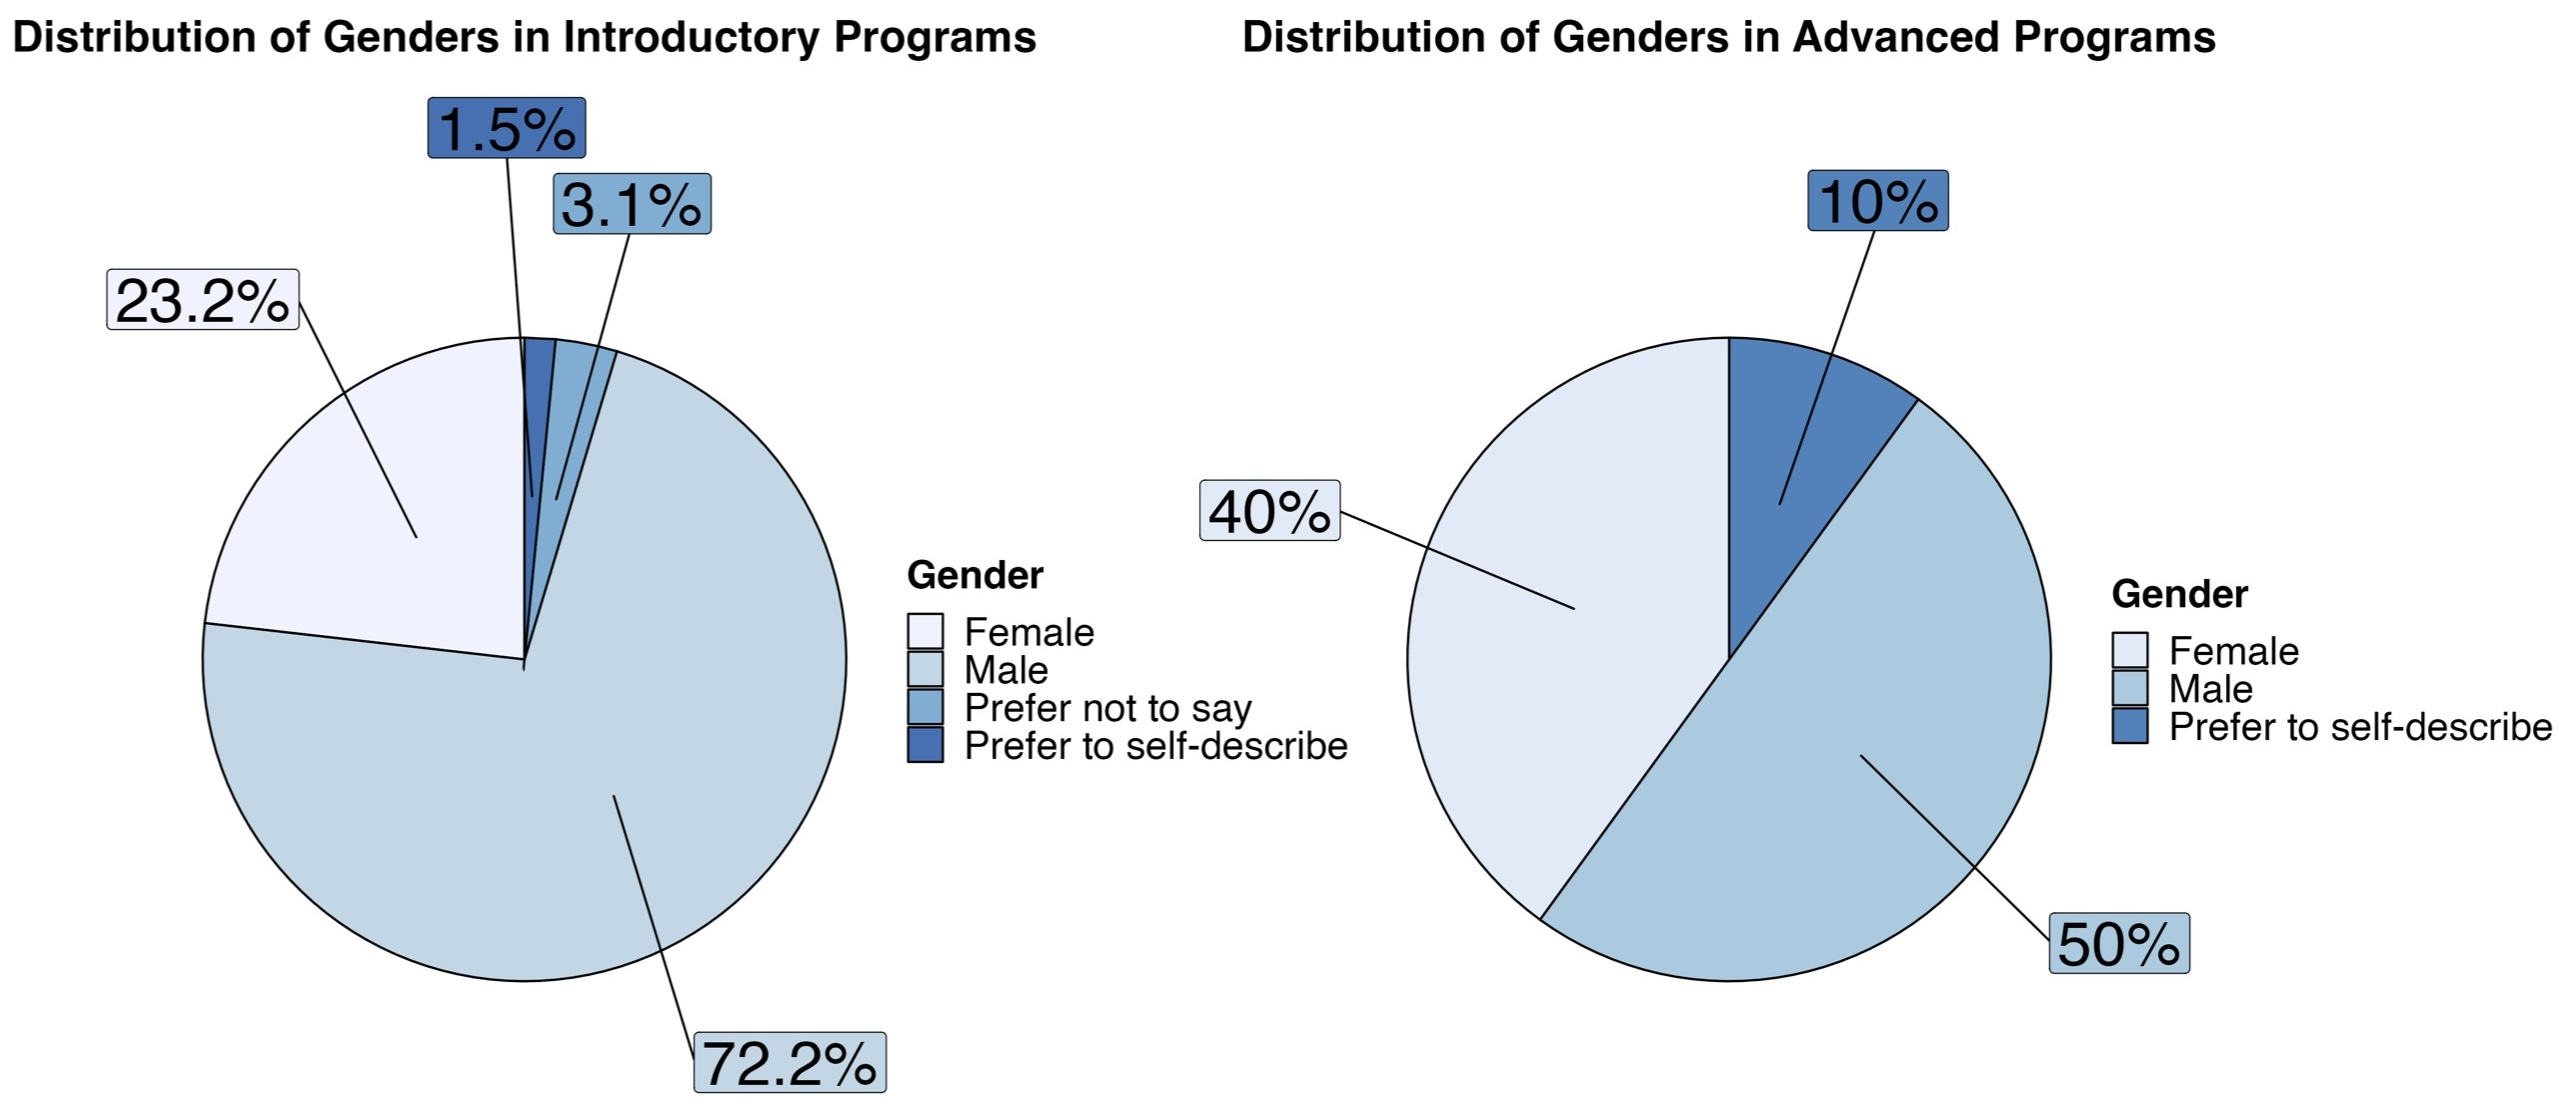
\includegraphics[width=0.85\textwidth,height=\textheight]{Graphs/Report/GGEE_23_Gender_IA.jpg}
\caption{\emph{The distribution of students genders for the introductory
(left, n=194) and advanced (right,n=10) Goldberg Gator Engineering
Explorer Summer Programs}}
\end{figure}

\hypertarget{race-and-ethnicity}{%
\subsubsection{Race and Ethnicity}\label{race-and-ethnicity}}

In the Pre-survey, students were given the option to select as many
options apply to them from the following list: American Indian/Alaskan
Native, Asian, Black or African American, Hispanic or Latin(x), Native
Hawaiian or other Pacific Islander, or White. Most students chose one to
two options to classify their race and ethnicity. In order to evaluate
the distribution of students across the programs, students that listed 3
or more race/ethnicity options were grouped together. There were 7
students out of the 204 surveyed that chose 3 or more options. Those
results were as follows:

\begin{itemize}
\tightlist
\item
  1 student American Indian or Alaska Native, Black or African American,
  and White
\item
  2 students Hispanic or Latin(x), American Indian or Alaska Native, and
  White
\item
  1 student Hispanic or Latin(x), Asian, and Black or African American
\item
  2 students Hispanic or Latin(x), Asian, and White
\item
  1 student that selected all options
\end{itemize}

To display the distribution of student race and ethnicity, the results
were displayed as a total number of students that selected a race or
ethnicity with the number of students who chose a specific secondary
race or ethnicity within the bar of the graph.

The distribution or race and ethnicity for all GGEE summer programs is
shown in Figure 10. Of the 204 students surveyed, 44.1 percent of
students (90 students) selected White as their race. 84 students
selected just White while other 6 students selected both White and
Hispanic/Latinx. 13.2 percent of students (27 students) selected
Hispanic/Latinx. 24.5 percent of students (50 students) selected Black
or African American as their race. 43 students identified as Black or
African American, 3 students selected Black or African American and
White, and 4 students selected Black or African American and
Hispanic/Latinx. 12.7 percent of students (26 students) identified as
Asian, 21 students only selected Asian while 1 student selected Asian
and Black or African American, and 2 students selected both White and
Asian or White and Hispanic/Latinx. 2 percent of students (4 students)
selected American Indian or Alaska Native with 2 students solely
selecting American Indian or Alaska Native, 1 student selected American
Indian or Alaska Native and Asian, and 1 student selected American
Indian or Alaska Native and Hispanic/Latinx. 3.4 percent or 7 students
selected more than 3 race/ethnicity options.

\begin{figure}
\centering
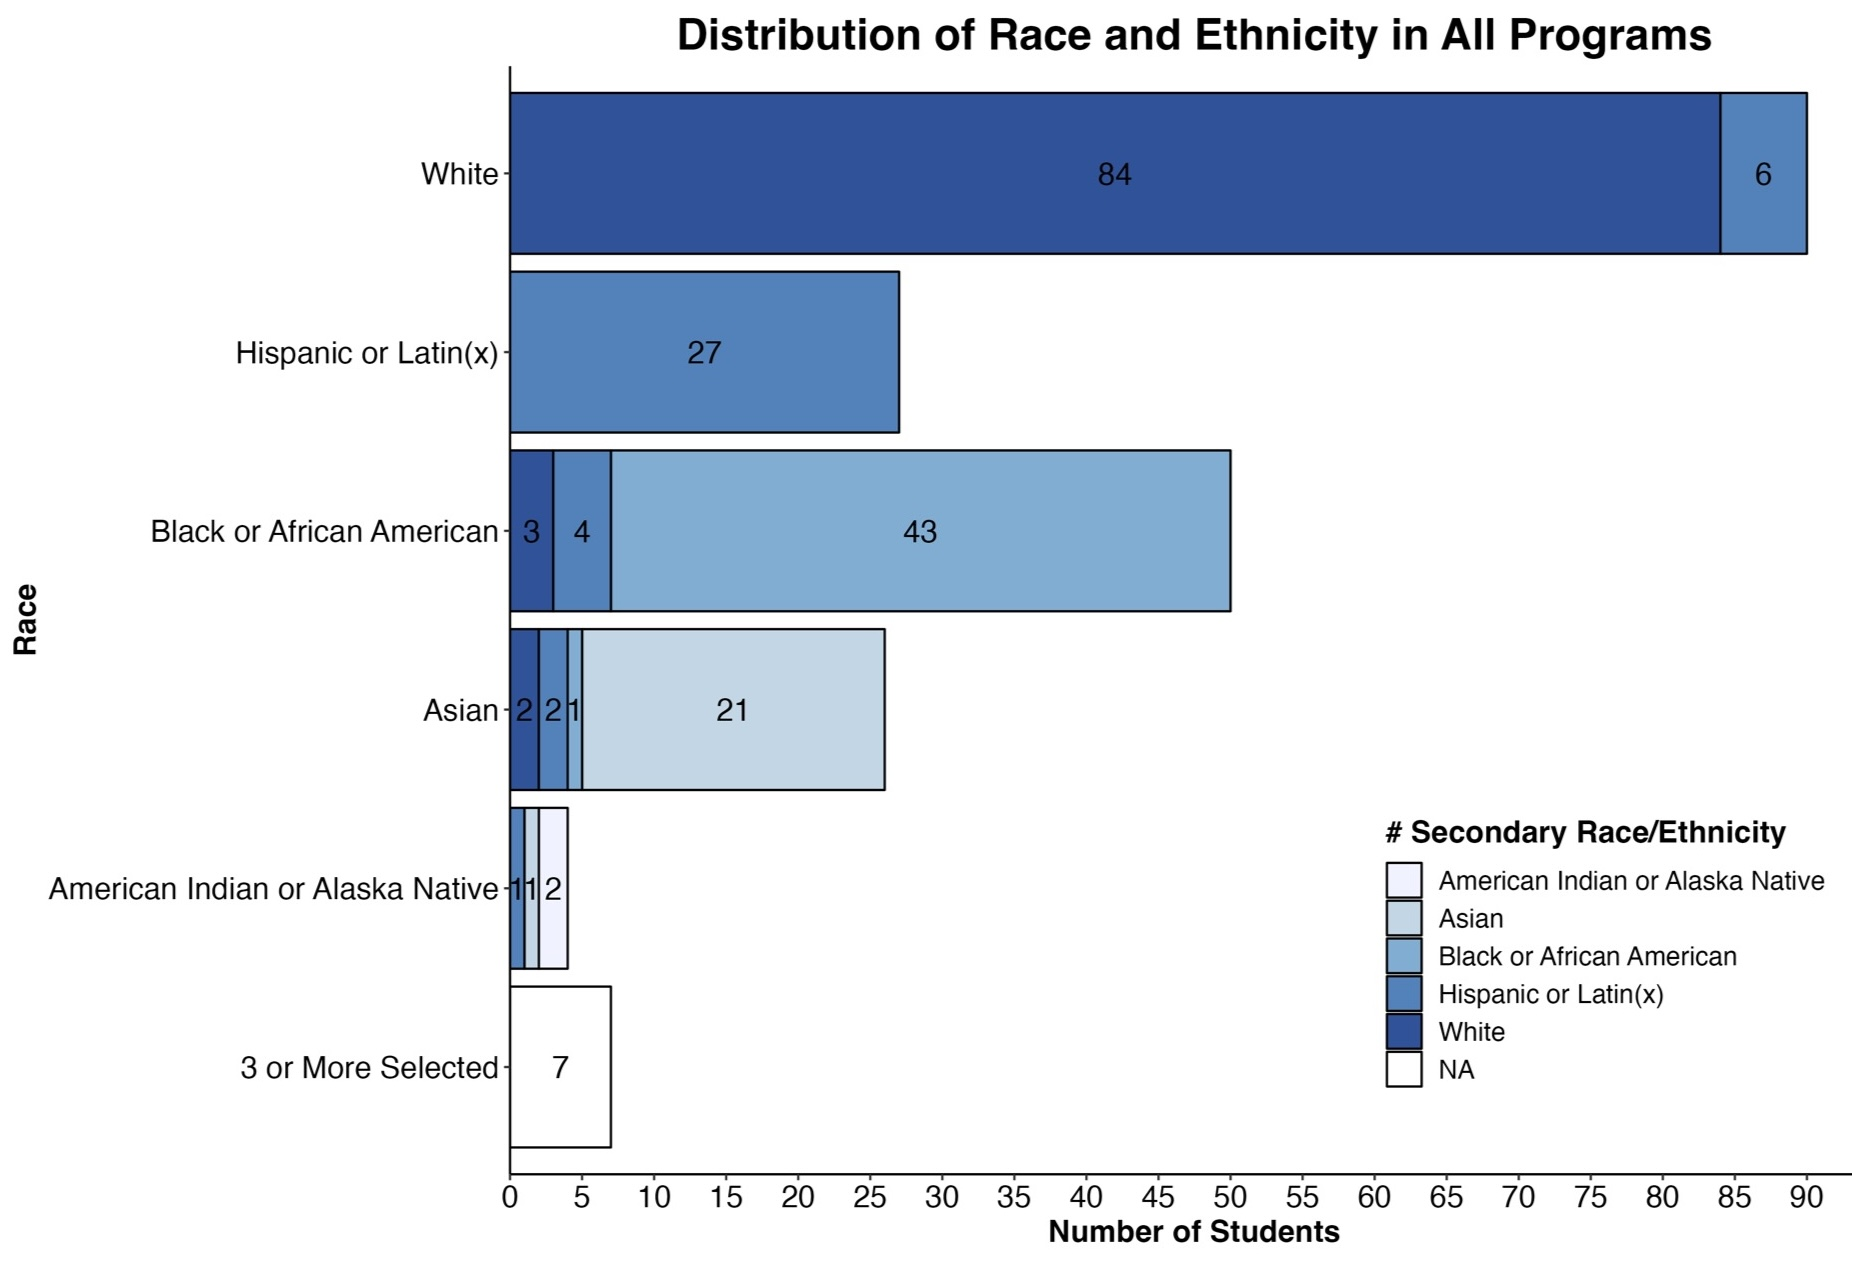
\includegraphics[width=0.7\textwidth,height=\textheight]{Graphs/Report/GGEE_23_Race_All_Num.jpg}
\caption{\emph{The distribution of student race and ethnicities for both
introductory and advanced Goldberg Gator Engineering Explorer Summer
Programs (n=204)}}
\end{figure}

In the introductory programs there was a similar distribution of student
race and ethnicity compared to both programs combined, Figure 11. Of the
194 students, 44.8 percent of students (87 students) selected White as
their race. 82 students selected White and 5 students selected White and
Hispanic/Latinx. 13.4 percent of students (26 students) selected
Hispanic/Latinx. 24.2 percent (47 students) chose a race including Black
or African American. 42 students selected Black or African American, 3
students selected Black or African American and Hispanic/Latinx, and 2
students selected Black or African American and White. 12.4 percent of
students (24 students) identified as Asian; 19 selected Asian, 2
selected Asian and Black or African American, 2 selected Asian and
Hispanic/Latinx, and 1 selected Asian and White. 2.1 percent of students
(4 students) chose an option including American Indian or Alaska Native.
2 students chose American Indian or Alaska Native, 1 student chose
American Indian or Alaska Native and Asian, and 1 student chose American
Indian or Alaska Native and Hispanic/Latinx.

\begin{figure}
\centering
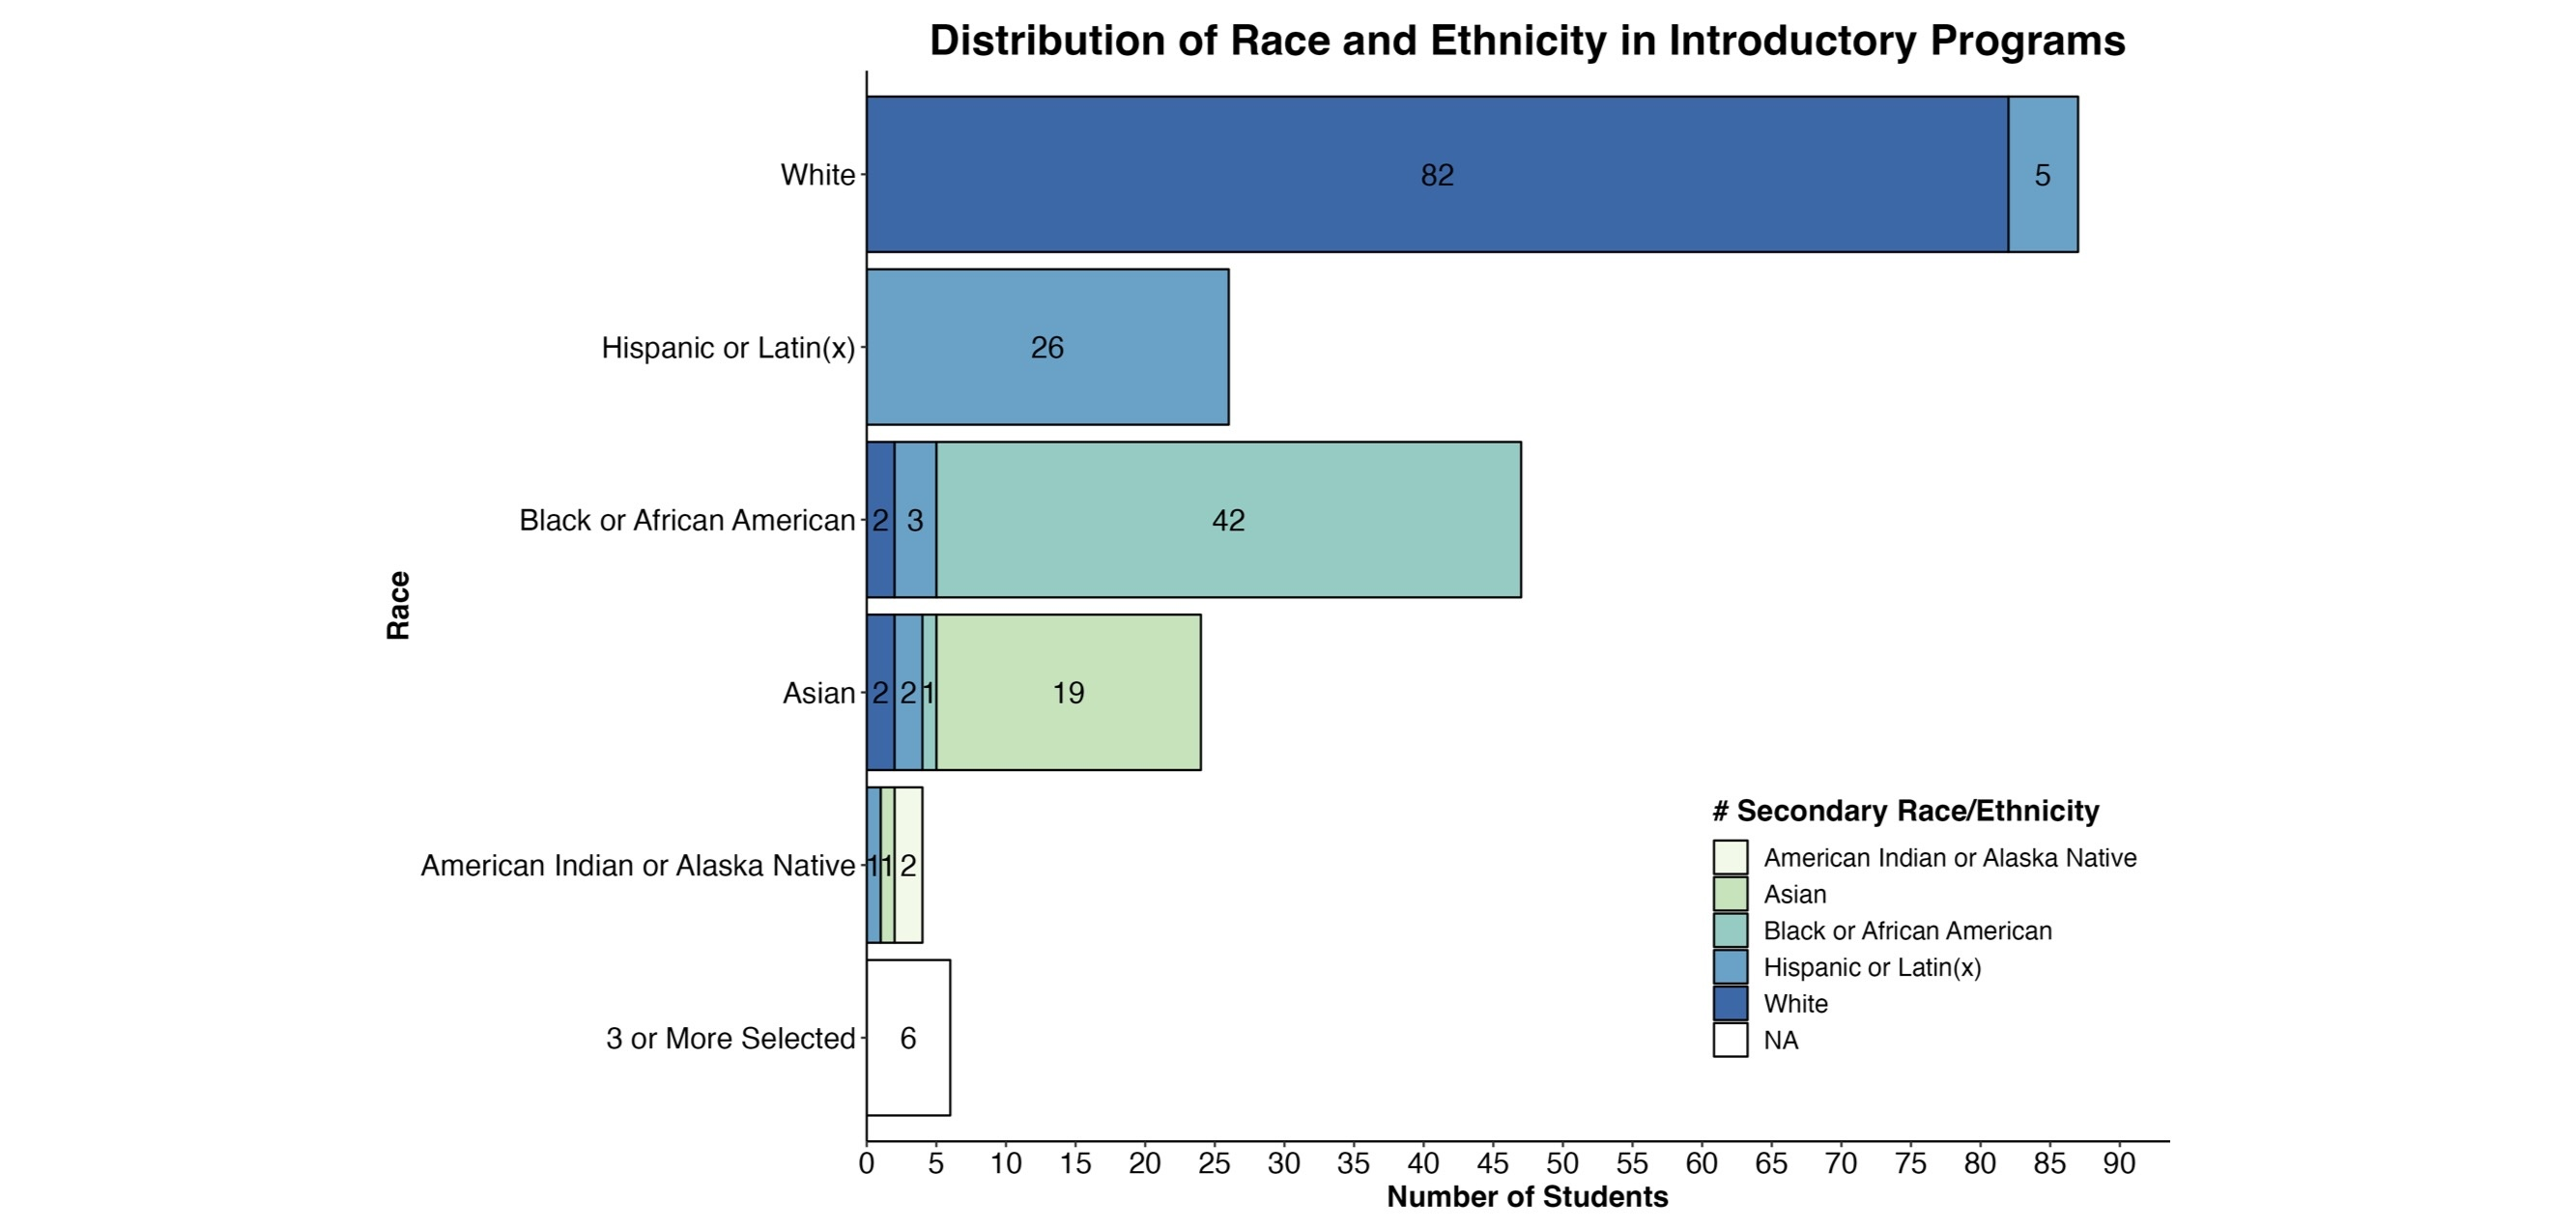
\includegraphics[width=0.7\textwidth,height=\textheight]{Graphs/Report/GGEE_23_Race_In_Num.jpg}
\caption{\emph{The distribution of student race and ethnicities for
Introductory Goldberg Gator Engineering Explorer Summer Programs
(n=194)}}
\end{figure}

Of the 10 students that participated in the research study for the
advanced program, Figure 12, 30 percent (3 students) identified as
White; 2 students selected White while 1 student chose White and
Hispanic/Latinx. 10 percent (1 student) identified as completely
Hispanic/Latinx. 30 percent of students (3 students) identified as Black
or African American; 1 student chose Black or African American, 1
student chose Black or African American and White, and 1 student chose
Black or African American and Hispanic/Latinx. 20 percent (2 students)
identified as Asian and 10 percent (1 student) chose more than 3
race/ethnicity options to identify themselves.

\begin{figure}
\centering
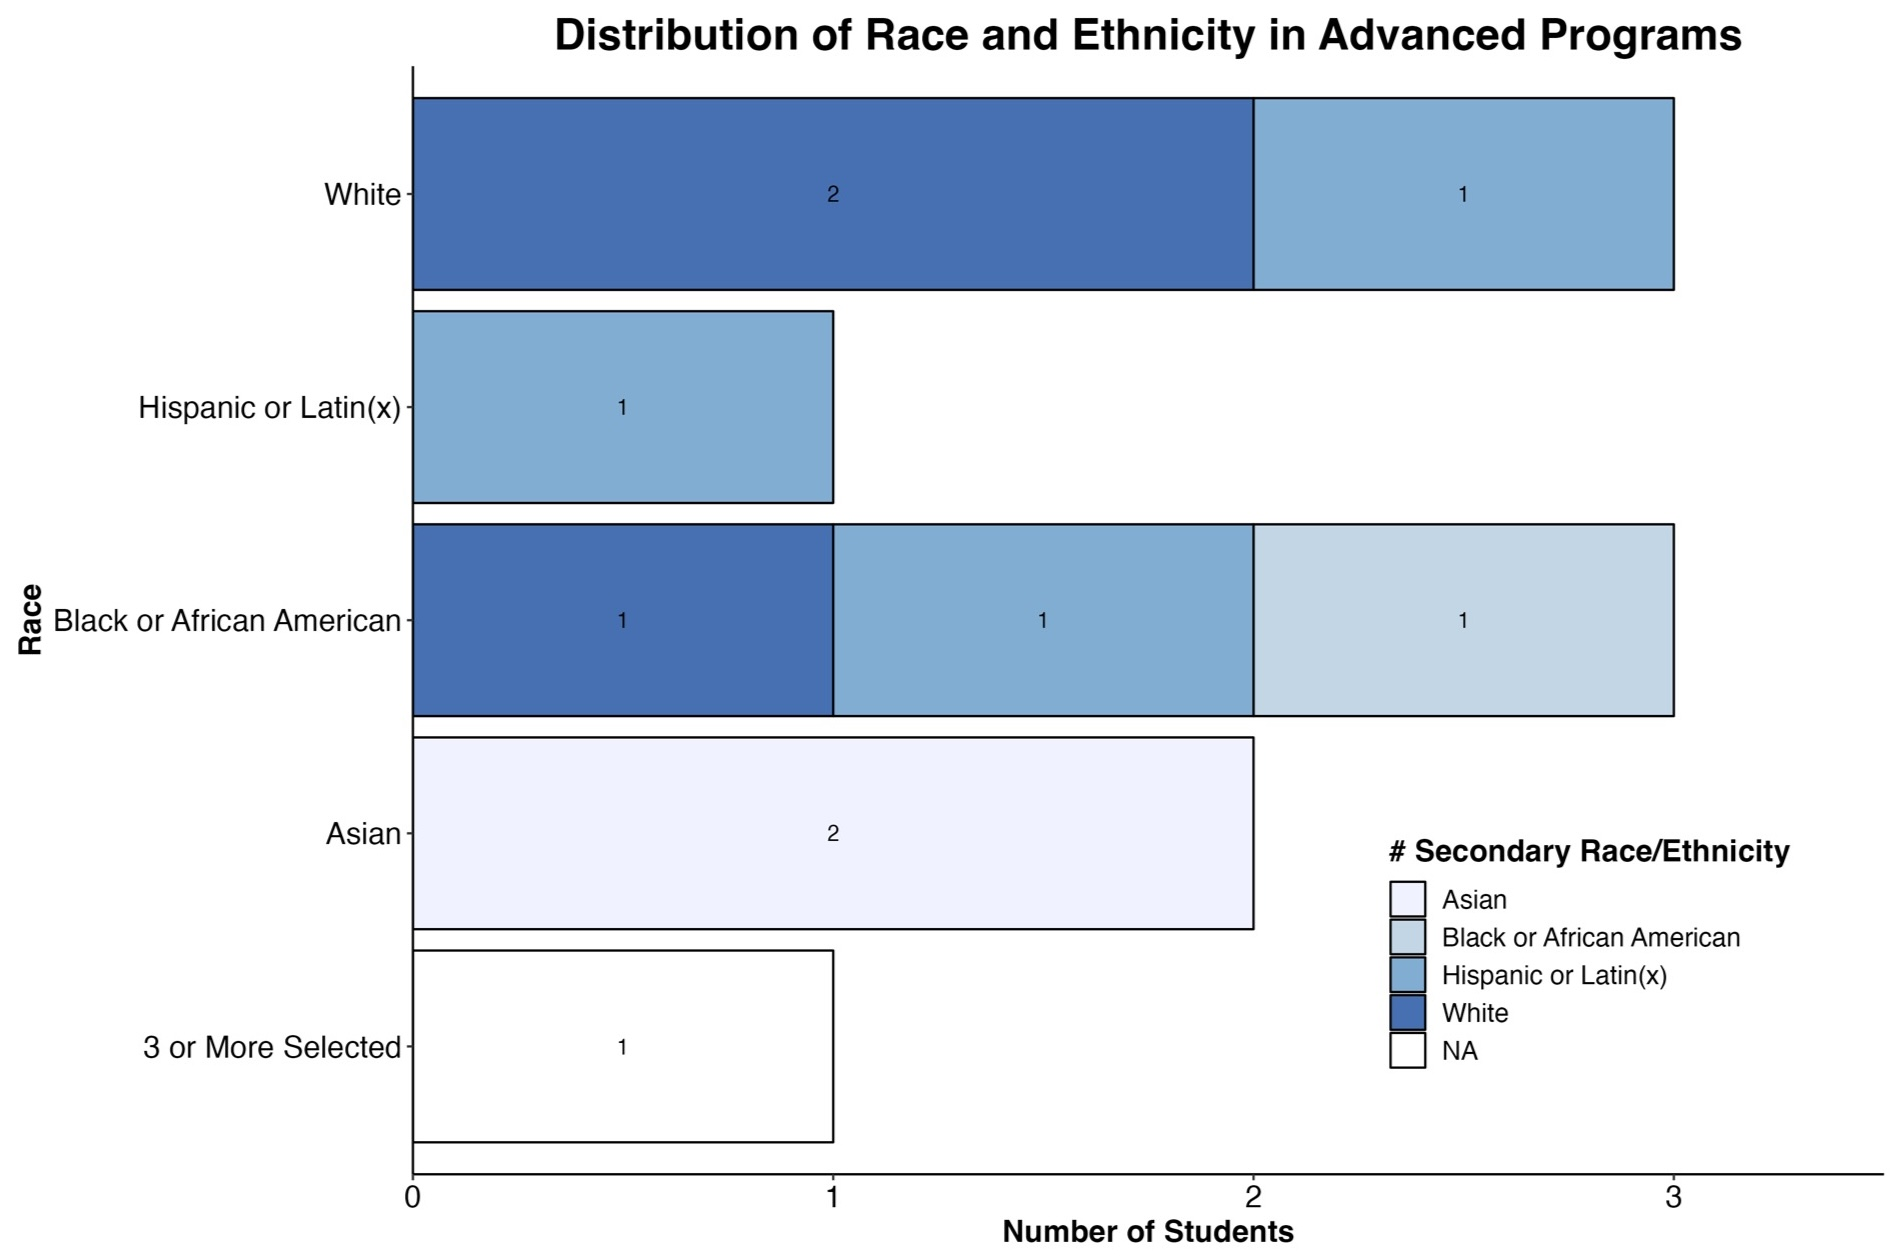
\includegraphics[width=0.7\textwidth,height=\textheight]{Graphs/Report/GGEE_23_Race_Adv_Num.jpg}
\caption{\emph{The distribution of student race and ethnicities for
Advanced Goldberg Gator Engineering Explorer Summer Programs (n=10)}}
\end{figure}

\hypertarget{ongoing-research}{%
\section{Ongoing Research}\label{ongoing-research}}

Analysis of the data collected from surveys and interviews during the
2023 GGEE summer program are in progress. We anticipate to have the
results from pre and post program particiaption as well as complete
thematic analysis for both 2022 and 2023 sessions by December 2023.

\hypertarget{student-surveys}{%
\subsection{Student Surveys}\label{student-surveys}}

\hypertarget{pre-survey}{%
\subsubsection{Pre-Survey}\label{pre-survey}}

The pre-survey was taken by students on the first day of the program.
Students were asked about their demographic information. They were asked
``How much experience did you have with coding or programming before the
camp?'' by selecting from ``No Experience'', ``A Little Experience'',
``Some Experience'', ``A lot of Experience.'' Students were also asked
to rate their coding skills before the summer program using the
following scale: 0 - None, 1 - Basic, 2 - Medium, 3 - High. Students
described what their prior experiences with programming were in order to
get a better picture of student's prior programming experiences. A world
cloud was generated using words that occurred more than once in student
responses, Figure 13.

For the advanced programs, students were asked about their prior
experiences with artificial intelligence, what those prior experiences
were, and the level that they enjoyed artificial intelligence.

\begin{figure}
\centering
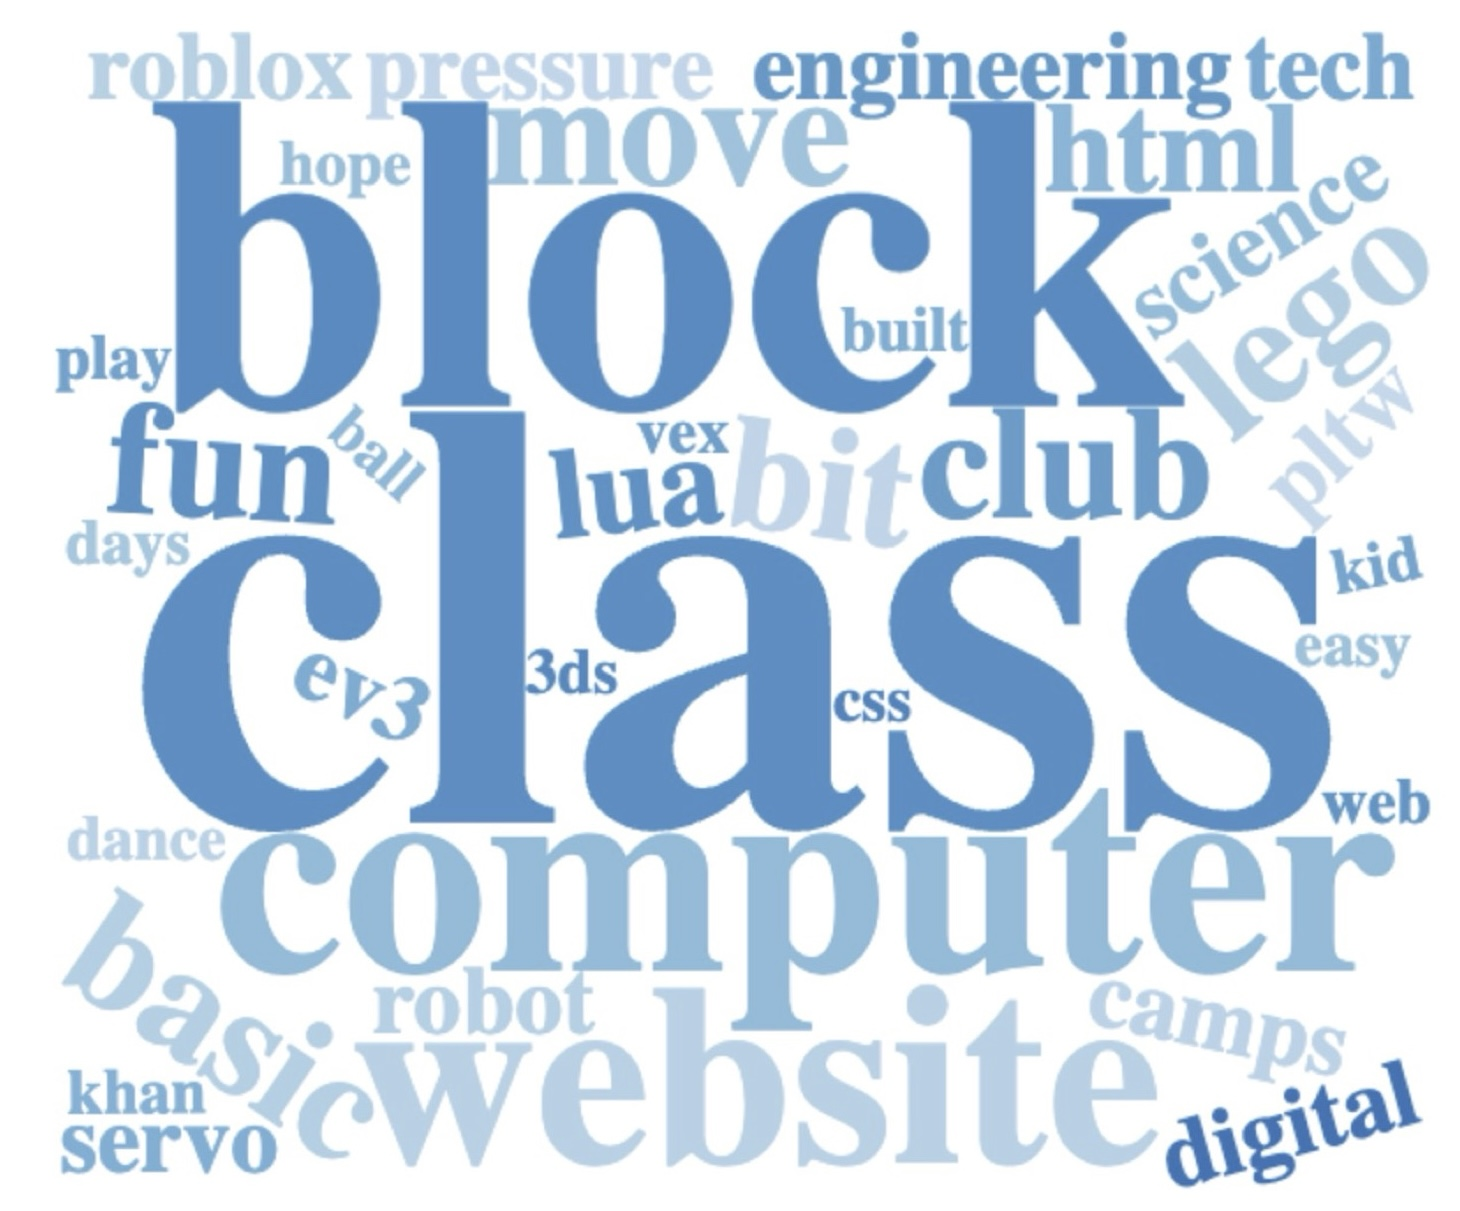
\includegraphics[width=0.6\textwidth,height=\textheight]{Graphs/Report/GGEE_23_WordCloud.jpg}
\caption{\emph{A word cloud generated from introductory program student
responses around the types of prior programming experiences they have
had.}}
\end{figure}

\hypertarget{end-of-day-survey}{%
\subsubsection{End of Day Survey}\label{end-of-day-survey}}

At the end of each day, students completed an end of day survey to
capture their experiences as the activities increased in difficulty from
beginning programming to engineering design projects.

Students were asked to rank the following questions on a 5-point Likert
scale ranging from strongly disagree, somewhat disagree, neither agree
or disagree, somewhat agree, strongly agree.

\begin{itemize}
\tightlist
\item
  I felt confident when completing today's camp activities.
\item
  I enjoyed completing today's camp activities.
\item
  I find today's camp activities interesting.
\item
  I find today's camp activities difficult.
\item
  I felt successful after completing today's camp activities.
\item
  Today's camp activities made me feel like I was a computer scientist.
\item
  Today's camp activities are useful for what I will be doing in school.
\item
  Today's camp activities are useful for my future career goals.
\item
  I want to do more activities similar to today's camp activities.
\end{itemize}

In the surveys, students were given space to share about working with
their teams as well as a place to provide feedback on the activities
they completed during the program that day.

\hypertarget{end-of-program-survey}{%
\subsubsection{End of Program Survey}\label{end-of-program-survey}}

The End of Program survey serves as post survey for the program. This
survey was taken by students upon completion of the last activity at the
end of the summer program.

Students were asked the same questions from the pre-survey, ``How much
experience did you have with coding or programming before the camp?''
Students were given options from ``No Experience'', ``A Little
Experience'', ``Some Experience'', ``A lot of Experience''. Students
were also asked to rate their coding skills before the summer program
and after the summer program using the following scale: 0 - None, 1 -
Basic, 2 - Medium, 3 - High.

Just like the end of day surveys, students were asked to rank the
following questions on a 5-point Likert scale ranging from strongly
disagree, somewhat disagree, neither agree or disagree, somewhat agree,
strongly agree.

\begin{itemize}
\tightlist
\item
  I felt confident when completing today's camp activities.
\item
  I enjoyed completing today's camp activities.
\item
  I find today's camp activities interesting.
\item
  I find today's camp activities difficult.
\item
  I felt successful after completing today's camp activities.
\item
  Today's camp activities made me feel like I was a computer scientist.
\item
  Today's camp activities are useful for what I will be doing in school.
\item
  Today's camp activities are useful for my future career goals.
\item
  I want to do more activities similar to today's camp activities.
\end{itemize}

\hypertarget{student-interviews}{%
\subsection{Student Interviews}\label{student-interviews}}

Students were interviewed in person and virtually once during the
duration of the summer program. Students were de-identified by assigning
a number to their name and recording the responses according to their
number. This is done to avoid bias when assessing the responses.

During the interview students were asked four questions to learn more
about their experience in the program and motivation to participate in
the program. Students were asked to respond to the following questions:

\begin{itemize}
\tightlist
\item
  Describe your experiences in completing the camp activities.
\item
  What has been challenging for you during the camp?
\item
  What have you learned as a result of the camp activities?
\item
  Why did you decide to try this or do this?
\end{itemize}

When analyzing the interviews from the pilot summer programs, a
sentiment analysis was completed to get a general picture of how
students felt in regard to the participating in the summer program. To
analyze student interviews further, a thematic analysis will be
completed for both 2022 and 2023 summer programs. Thematic analysis will
identify and quantify major themes in student responses to the interview
questions.

\hypertarget{teacher-interviews}{%
\subsection{Teacher Interviews}\label{teacher-interviews}}

Teachers were interviewed at the end of the summer programs. The
interview responses were also de-identified with random numbers to
prevent bias during analysis. A thematic analysis of the 13 teacher
interviews will be completed to identify any major themes and ideas that
arise in the interviews.

Teachers were asked the following questions during the interview:

\begin{itemize}
\tightlist
\item
  Describe your experiences in completing the camp activities.
\item
  How has your participation impacted the way you think about teaching?
\item
  How do you plan to incorporate computational thinking, engineering
  design, use of technology and system thinking in your future
  classrooms?
\end{itemize}

The goal of the interview was to see how teachers felt about the summer
programs and how the programs impacted their views on teaching and their
classroom practices.

\hypertarget{challenges-lessons-learned-and-modifications}{%
\section{Challenges, Lessons Learned, and
Modifications}\label{challenges-lessons-learned-and-modifications}}

\emph{Challenges faced, lessons leared, and adaptations.}

\begin{itemize}
\tightlist
\item
  Virtual Interviews - internet connection, authentic responses, quiet
  connected places for interviews
\item
  Virtual Observations - hard to tell what is going on in the classroom,
  no time to properly train students in observation protocols. Need to
  incorporate that into the training program in addition to learning the
  content
\item
  Student recruitment - delays from HR and confirmation of funding to
  support student mentors
\item
  Ensure no tasks are implied tasks for teacher prep - attendance,
  student drop off and pick up etc.
\item
  Parent documents - have the documents be a requirement for
  registration instead of having 2 surveys
\item
  Youth Compliance - uploading students and teachers in to the portal -
  identifying all required versus suggested information
\end{itemize}

\hypertarget{recommendations-for-program-improvement}{%
\section{Recommendations for Program
Improvement}\label{recommendations-for-program-improvement}}

\emph{Provide recommendations for improving the program in future
iterations, based on the insights gained.}

\begin{itemize}
\tightlist
\item
  Updating compliance forms with more clear language for parent and the
  research study
\item
  Make submitting paperwork a part of the registration process. Did this
  with the 2023-2024 After-School programs and it has made everything so
  much easier to process and collect rather than a 2-step process
\item
  Creating contract-like documents to denote needs, requirements, and
  expectations from the schools and what is provided from the GGEE
  program at UF
\item
  Starting Recruitment in November
\item
  working to recruit more female students into the intro summer programs
  by collaborating with the school districts and providing suggestions
  to recruit more female students into the program. -- does this look
  like videos, showing female students, changing the look of the flyers,
  working with teachers, focusing on girl clubs
\item
  ensuring districts cover technology to continue to use in after-school
  programs or integrate into classroom projects
\item
  revise research study to expand to get more teacher and UF
  undergraduate mentor insight in the program
\item
  more summer program options in Santa Rosa County - the students and
  families are interested in their students participating in the
  programs.
\end{itemize}

\hypertarget{after-school-programs}{%
\section{After-school Programs}\label{after-school-programs}}

\emph{Suggest potential directions for the program's growth or
expansion.}

After-school Programs

overview of programs

\hypertarget{conclusion}{%
\section{Conclusion}\label{conclusion}}

Summarize the program's achievements and positive outcomes.

Emphasize how the program benefited the participating students and the
broader school community.

\pagebreak

\hypertarget{appendices}{%
\section{Appendices}\label{appendices}}

\hypertarget{appendix-1-summer-program-calendar}{%
\subsection{Appendix 1: Summer Program
Calendar}\label{appendix-1-summer-program-calendar}}

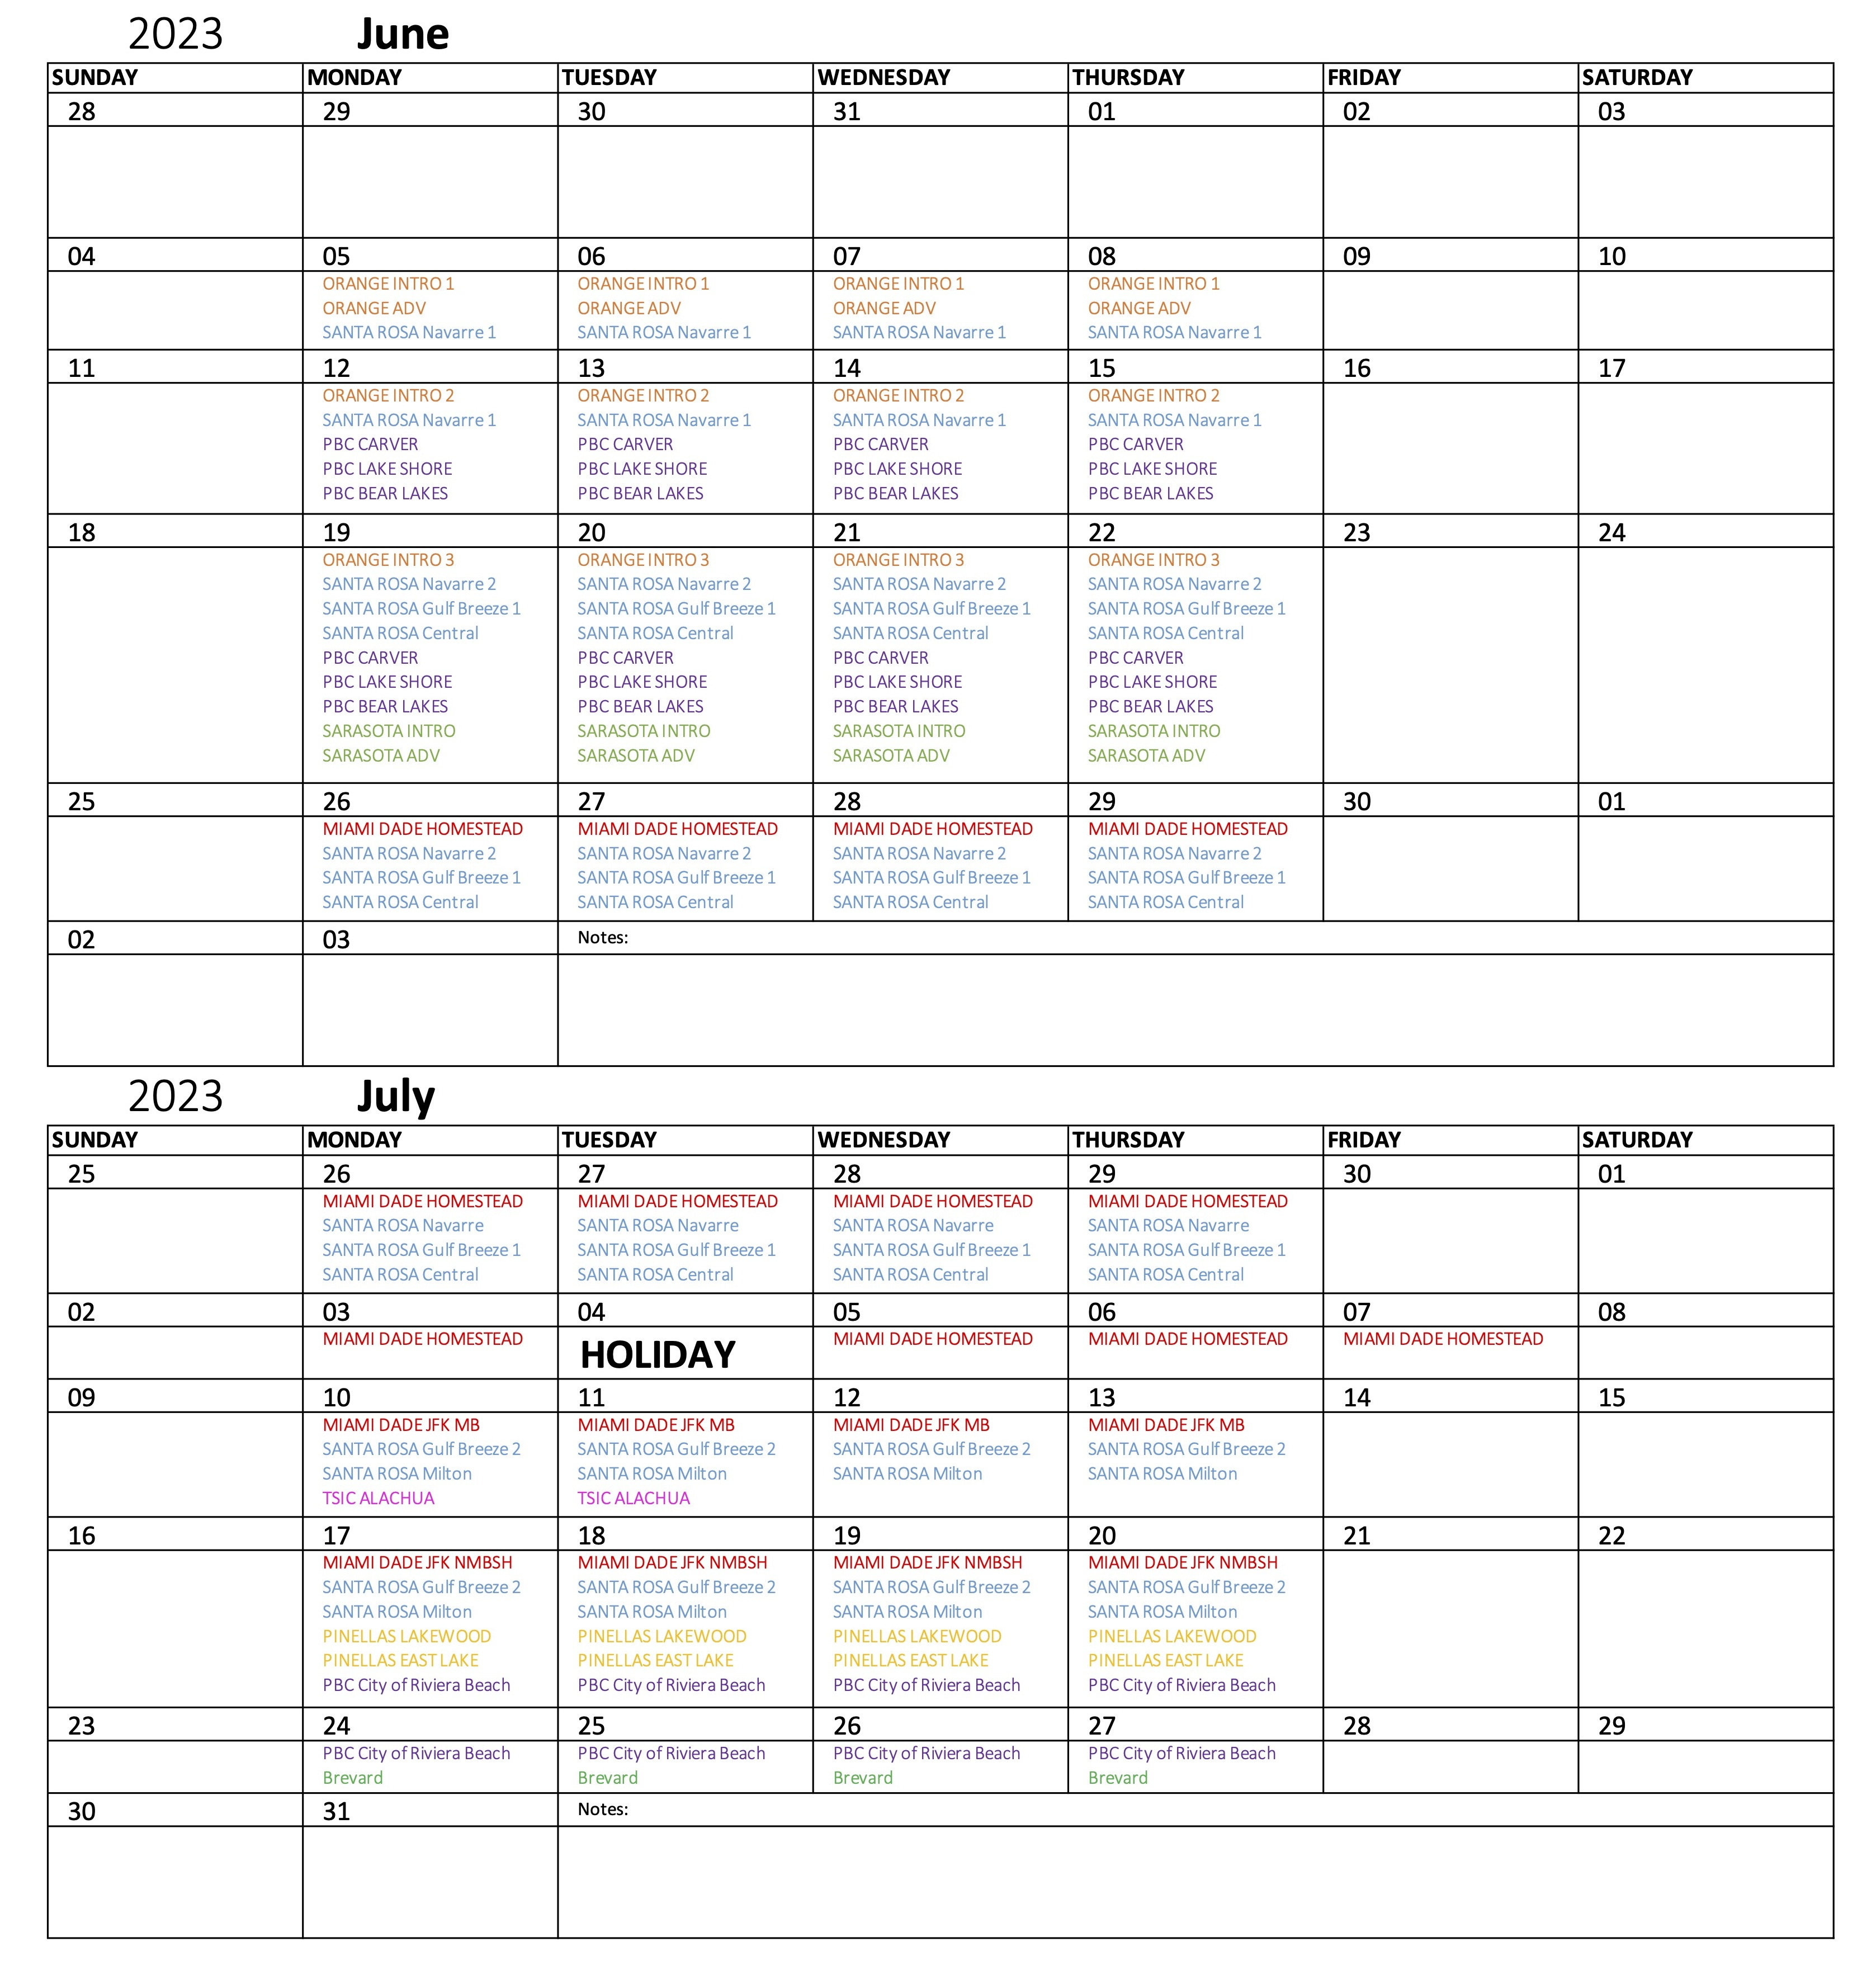
\includegraphics[width=1\textwidth,height=\textheight]{Images/GGEE_23_Calendar.jpg}

\end{document}
